\documentclass[doc,apacite,oneside,a4paper,12pt]{apa6}
\usepackage[T1]{fontenc}		% Selecao de codigos de fonte.
\usepackage{indentfirst}		% Indenta o primeiro parágrafo de cada seção.
\usepackage{nomencl} 			% Lista de simbolos
\usepackage{color}				% Controle das cores
\usepackage{graphicx}			% Inclusão de gráficos
\usepackage{microtype} 			% para melhorias de justificação
\usepackage{amsmath}
\usepackage{amsthm}
\usepackage{amsfonts}
\usepackage{setspace}
\usepackage[portuguese]{babel}
\usepackage{geometry}
\usepackage{ragged2e}
\usepackage{lscape}
\usepackage{array,multirow,graphicx}
\usepackage{graphicx}
\usepackage{mwe}
\usepackage{epstopdf}
\usepackage{subfig}
\usepackage{caption}
\usepackage{graphicx}
\usepackage{sidecap}
\bibliographystyle{bbs}
\usepackage{float}
\graphicspath{{images//}}

\usepackage{endnotes}
\renewcommand*{\notesname}{Notas}
\let\footnote\endnote


\usepackage{fancyhdr}
% Turn on the style
\pagestyle{fancy}
\fancyhead{}
\fancyfoot{}
\fancyfoot[R]{\thepage}

%Times new roman
%\usepackage{fontspec}
%\setmainfont{Times New Roman}
\usepackage{times}
\usepackage[portuguese]{babel}
\usepackage[utf8]{inputenc}

%Margens
\geometry{left=3cm,right=2cm,top=3cm,bottom=2cm}

%Citações
%\cite, \citeA, \citeNP
%s \citet and \citep, use double square brackets, for example,
%\citep[see][for more details]{ex1}.

\title{Premier League via Dirichilet Regression }
\shorttitle{Premier League via Dirichilet Regression}

\author{Nascimento, Igor Ferreira do}
\affiliation{Departamento de Administração - UnB; Laboratório de Aprendizado de Máquina em Finanças}

%%% Resumo do trabalho contendo até 250 palavras, no mesmo idioma do trabalho.
\abstract{O artigo apresenta uma metodologia para estimar a probabilidades dos resultados dos jogos da Premier League utilizando covariáveis dos jogadores.}


% Palavras-chave: até cinco palavras-chave.
\keywords{Regularization,Dirichilet Regression,Premier League,Forecast}


%\rightheader{APA style}
%\leftheader{Author One}

\begin{document}
\singlespacing 
\justify

\maketitle    
                        
\section{Introdução}
\label{sec:int}
\noindent

O fascínio por eventos incertos instiga o ser humano desde os remotos tempos dos antepassados. Os historiadores XXXX mostram que desde a época o ser humano demonstrava interesse por saber ao menos algo sobre o que é incerto. Ao longo dos anos, a teoria dos jogos proporcionou o desenvolvimento de modelos probabilísticos para determinar o nível de determinados ocorrências.



O objetivo do trabalho é apresentar modelos probabilísticos para representar os resultados da Premier League por meio de covariáveis relacionado ao capital humano do time e os recursos financeiros relacionados ao time. Além disso, é apresentado uma estimação para o resultado final da tabela de classificação.

\section{Sports Forecast}
\label{sec:foresport}
\noindent



Sport is a human activity normally related to the playful environment but we can not dissemble the betting. The work like \cite{Kain2014} analyse the dissonance between the outcome of sports and the sports betting market explained by fact the set betting lines is straight related with the profit goal instead the outcome probability. On the other hand, the  paper \cite{Strumbelj2010} analysed  some European soccer leagues and show that exist evidence that bookmakers learn over time about soccer prediction results. Anyway, this is interesting to either bettors or bookmakers researchers in this area.



Dito isso, pode-se destacar que os resultados esportivos possuem uma intenso interesse da sociedade como um toda, seja ela do ponto de vista financeiro ou a mera busca por entreternimento.



As redes de apostas como, XXX, YYY, GGG SÃO encontrados ao redor do mundo e fazem girar cifras ainda maiores de recursos no ato de acreditar em um determinado resultado. Esportes como o baiseball e o futebol americano possuem grande suporte dos cientistas de dados para apresentar pequenas melhoras nos resultados individuais dos atletas que aparentam ser inespressíveis, ao menos aos olhos dos descuidados, porém representam um grande impacto no coletivo e consequentemente, em toda a cadeia produtiva associada ao esporte. De encontro com tais anseios está o vertiginoso desenvolvimento de tecnologias de captação, armazenamento, tratamento e analise de dados relacionados às atividades esportivas.

O futebol é, se não o mais, um dos esportes com as movimentações de destaque na atualidade. Atualmente, existem elenco de jogadores em times que passam a casa dos 10 dígitos, sobre tudo na Europa Ocidental. Os times Espanhóis e Britânicos lideram os valores financeiros relacionados ao capital humano disponível. No entanto, essa aparente hegemonia é, cada vez mais, desafiada com o surgimento de novos mercados da bola. O mercado Norte Americano tem investido mais de XXXXX milhões de dólares em um projeto de incentivo à prática do futebol, desafiador em uma nação com outros esportes com importância sacramentada como é o caso do Futebol Americado e Basquete.

O evento mais recente e com maior destaque no mundo do esporte foi o valor total da transferência de Neymar do Barcelona para o Paris Saint German, um total de mais 400 milhões de euros. Seria ingenuidade não encarar tal transação como um investimento. É esperado que as externalidades dessa movimentação tenha reflexos comparadas com os maiores investimentos nos mercados de financeiros do mundo. Por exemplo, a venda de camisas aumentou $123123123321\%$ no faturamento do clube apenas com vendas de camisas.


\section{Regressão Dirichilet}
\label{sec:mod}
\noindent



A distribuição Dirichilet permite modelar um vetor composicional de dimensão $k\leq 2$ $Y = (y_1,y_2,\cdots,y_K)$, com parâmetros de escala $\alpha_1,\alpha_2,\cdots,\alpha_K\geq 0$, sendo $\sum_{j=1}^K y_j = 1$ um padrão $K-1$ simplex. Dessa forma, as probabilidades presentes na distribuição multinomial tem como priori conjugada tal distribuição, com densidade probabilidade:

The Dirichilet distribution is able to model a composite vector of dimension $k\leq 2$ $Y = (y_1,y_2,\cdots,y_K)$, with scalings parameters $\alpha_1,\alpha_2,\cdots,\alpha_K\geq 0$ , being  $\sum_{j=1}^K y_j = 1$ a standard $K-1$ simplex. Thus the probabilities present in the multinomial distribution have as a priori conjugated such distribution, with probability density:


\begin{equation}
P(Y |\alpha) = \frac{\prod_{j=1}^K\Gamma(\alpha_j)}{\Gamma(\sum_{j=1}^k\alpha_j)}\prod_{j=1}^K y^{\alpha_j - 1}
\end{equation}


The work of \cite{Hijazi2009} that observed a good ajust upon longitudial covariates changes using Dirichilet Regression. In field of sports the work of \cite{Null2009} show a competitive accuracy modeling player abilities in Major League Baseball.

We object model the scale parameters by covariates $X_r$, and use this covariates to forecast the final classification result. Thus the model is:

\begin{equation}
g[\alpha_j(X)] =  \beta_{j0} + \beta_{j1} X_1 + \beta_{j2} X_2 + ... + \beta_{jR} X_R + \varepsilon_{j}
\label{eq:g}
\end{equation}

Being $g(.) = log(.)$  has a transformation possible.  The sample $Y$ with size $N$ the likelihood is:

\begin{equation*}
 L(\beta|X,Y) = \prod_{i=1}^N\left[ \frac{\prod_{j=1}^K\Gamma\left(\alpha_j(X)\right)}{\Gamma\left(\sum_{j=1}^k\alpha_c(X)\right)}\prod_{j=1}^K y_{ij}^{\alpha_j(X) - 1}\right]
 \end{equation*}
 

The coefficients $\beta_{jr}$ in each $\alpha_j$ of Equation \ref{eq:g} could be mensured solvind the minimum problem as.

\begin{equation}
\begin{aligned}
& \underset{\beta}{\text{maximize}}
& &   log(L(\beta|X,Y)) - \lambda\left[\phi(||\beta||) + (1-\phi)(||\beta^2||)\right]
\end{aligned}
\label{eq:vero}
 \end{equation}
 
 Being
 
\begin{equation*}
 log(L(\beta|X,Y)) = \sum_{i=1}^N log\left[\Gamma\left(\sum_{j=1}^K\alpha_j(X_{ri})\right)\right]	-\sum_{j=1}log\left[\Gamma\left(\alpha_j(X_{ri})\right)\right] + \sum_{j=1}^K[1-\alpha_j(X_{ri})]log\left(Y_{ji}\right)
 \label{eq:objfunc}
 \end{equation*}


Thus, we using a maximization procedure to find the $\beta$ coefficients in equation \ref{eq:g}.

Nosso modelo, $K=3$, sendo $\alpha_{Home}$ o parâmetro associado a probabilidade do time mandante vencer, $\alpha_{Visitor}$ a probabilidade do time visitante vencer e $\alpha_{Tie}$ a probabilidade para o empate dos times.

As variáveis regressoras são apresentadas a seguir. 

\section{Base de dados}
\label{sec:data}


Foram consideradas como regressoras as habilidades encontradas no site do jogo virtual FIFA. São elas \textbf{Aceleração},  \textbf{Altura},  \textbf{Cabeceio},  \textbf{Carrinho},  \textbf{Ch.},  \textbf{de},  \textbf{longe},  \textbf{Cobr.},  \textbf{falta},  \textbf{Combativ.},  \textbf{Contr.},  \textbf{bola},  \textbf{Cruzamento},  \textbf{Div.},  \textbf{em},  \textbf{pé},  \textbf{Dribles},  \textbf{Duração},  \textbf{Do},  \textbf{Contrato},  \textbf{Elast.},  \textbf{GL},  \textbf{Finalização},  \textbf{Fôlego},  \textbf{Força},  \textbf{Força},  \textbf{chute},  \textbf{Idade},  \textbf{Lançamento},  \textbf{Manejo},  \textbf{Marcação},  \textbf{Passe},  \textbf{curto},  \textbf{Perna},  \textbf{boa},  \textbf{Perna},  \textbf{ruim},  \textbf{Peso},  \textbf{Pique},  \textbf{pos},  \textbf{Posicion.},  \textbf{GL},  \textbf{Reação} e  \textbf{Reflexos}.

Foram coletadas informações durante o período de $2008$ e $2016$.


Similarmente ao \textit{Premier League}, os dados dos disponibilizados no site da FIFA acompanham os times de cada temporada. Os dados são atualizados mais de uma vez durante semana de jogos e foram considerados os valores da versão mais atualizada de cada temporada.


\begin{figure}%
    \centering
    \subfloat[\scriptsize{Summary acceleration mensures by match result.}]{{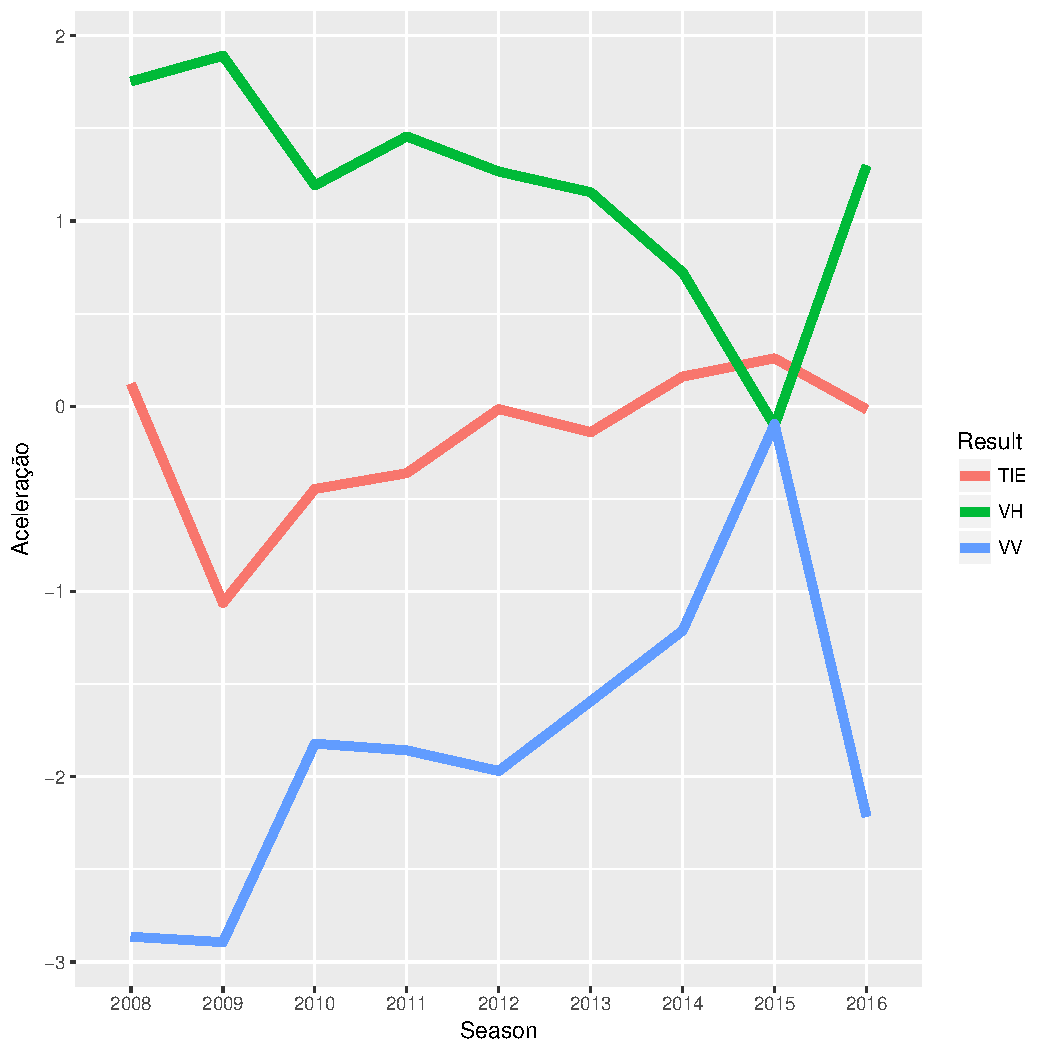
\includegraphics[width=5cm,height=4cm]{aceleracao_result.pdf} }}%
    \qquad
    \subfloat[\scriptsize{Acceleration mensure for period of analysis.}]{{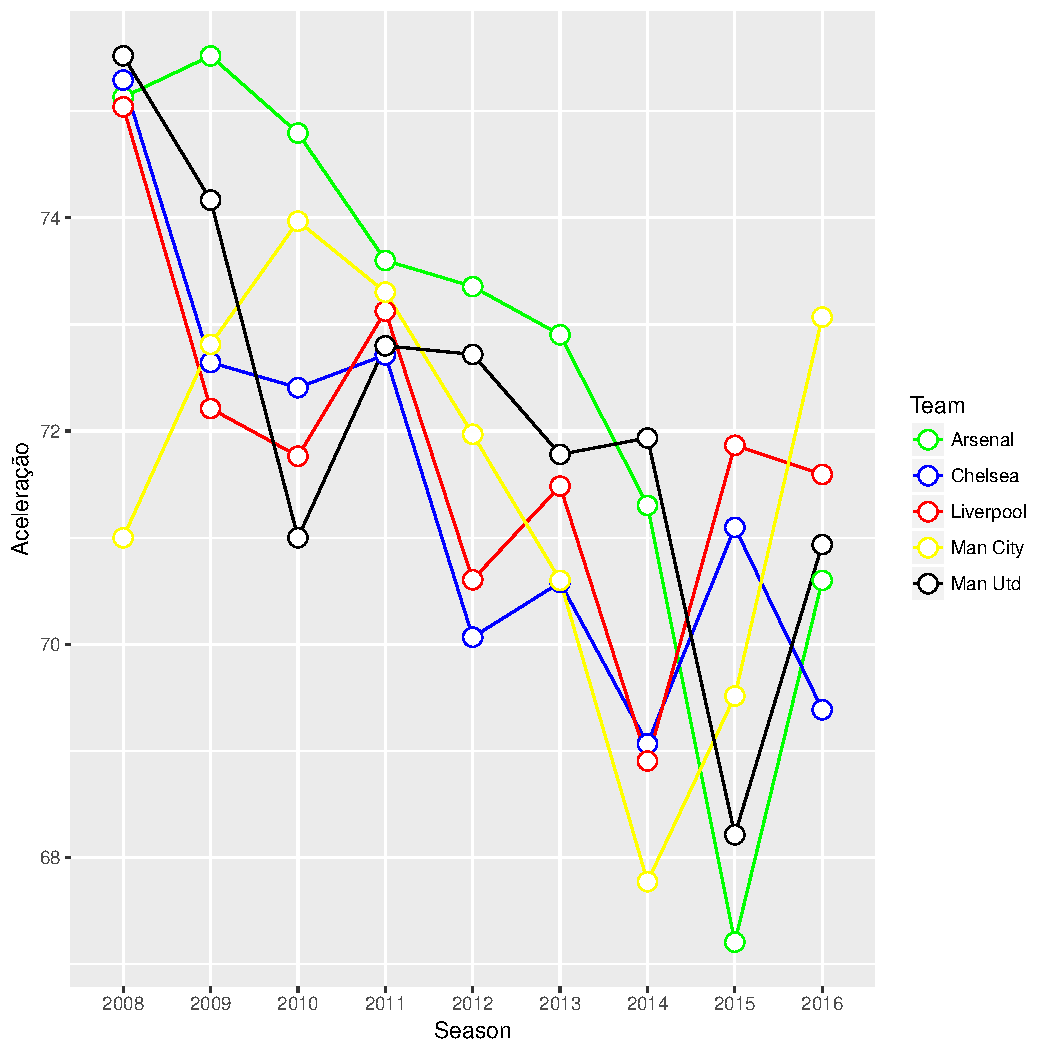
\includegraphics[width=5cm,height=4cm]{aceleracao_descri.pdf} }}%
    \caption[\scriptsize{Summary acceleration mensure.}]{\scriptsize{ \textbf{(a)} Summary acceleration mensures by match result. Tie (TIE), Victory of Home team (VH) and Victory of visitor team (VV). \textbf{(b)} Skill acceleration mensure for period of analysis. }}
    \label{fig:summary}%
\end{figure}


Seja $X^{home}_{r}$ o valor da veriável regressora $r$ para o time mandante do confronto e, analogamente, $X^{visitor}_{r}$ o valor para a mesma variável do time visitante. A equação do modelo \ref{eq:g} é modelada pela diferença entre a habilidade na variável $r$ entre o time mandante e o visitante. $X_{r} = X^{home}_{r}-X^{visitor}_{r}$. Dessa forma, valores muito positivos para a variável $X_{r}$ significam superioridade do time mandante e os negativos significam que as habilidades do time visitante são superiores aos anfitriões.


O gráfico do painel $(a)$ da imagem \ref{fig:summary} mostra que, em média, os jogos em que a medida $X_r$ é maior do que zero, houve vitória do time mandante. Do forma similar, nos casos em que $X_r$ foi menor do que zero o time visitante venceu. Os casos tem empate, há equilíbrio entre os times e a medida $X_r$ é próxima, em média, de zero. Em anexo estão as medidas para as demais variáveis.

O gráfico do painel $(b)$ da imagem \ref{fig:summary} mostra a evolução da variável aceleração ao longo do período de análise para os principais times da \textit{Premier League}. É possível perceber que todos times tiveram entre $2008$ e $2014$ uma diminuição do valor médio da variável aceleração. O processo de renovação de elenco do Chelsea, Liverpool e Mancherster City iniciou-se em $2015$. Já para Arsenal e Mancherster United a renovação ocorreu no ano seguinte em $2015$.

O início de renovação do Chelse foi campeã pode ajudar a explicar o sucesso em $2015$ e $2017$. Uma queda dessas e outras informações das equipes inglesas podem ajudar a compreender a zebra de $2016$, quando a equipe de pouca expressão Leicester foi campeã. 

Pretendemos explicar e predizer o resultado dos jogos da Premier League, baseado nas habilidades auferidas pelo site FIFA dos jogadores de cada time.

\section{Método}
\label{sec:metodo}

A base de dados foi dividia em:
\begin{itemize}
\item \textbf{base de treino:} jogos das temporadas de $2008$ e $2014$. A base servirá para estimar os parâmetros do modelo da equação \ref{eq:g}.
\item \textbf{base de tuning:} jogos das temporadas de $2015$. A base servirá para estimar os parâmetros $\lambda$ e $\phi$ do processo de \textbf{regularização} na equação \ref{eq:vero}.
\item \textbf{base de teste:} jogos das temporadas de $2016$. A base servirá para avaliar $out-of-sample$ o modelo.
\end{itemize}


Os parâmetros de $\phi$ e $\lambda$ foram avalidados por meio do \textit{grid-search}, sendo $\phi = (0 , 0.1,0.2,0.3,\cdots,0.9,1)$ e  $\lambda =( 0,0.5,1,1.5,2,2.5,3)$. Os gráficos da figura \ref{fig:tunning} apresentam o desempenho do modelo para o \textit{grid} de procura dos parâmetros.


\begin{figure}%
    \centering
    \subfloat[\scriptsize{Tunning surface parameters}]{{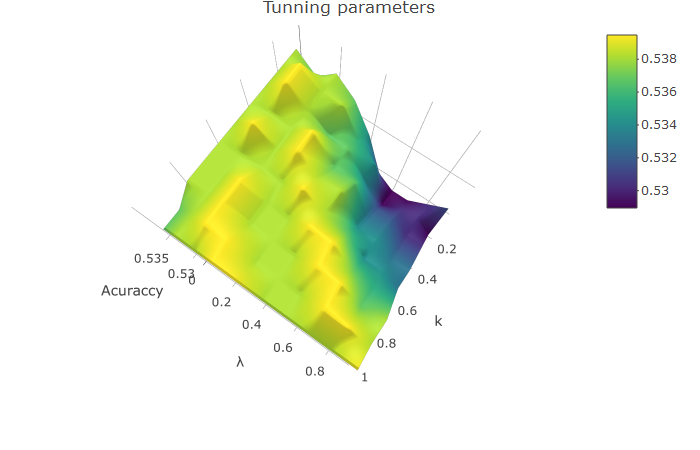
\includegraphics[width=5cm,height=4cm]{tunning_all.png} }}%
    \qquad
    \subfloat[\scriptsize{Tunning contour parameters }]{{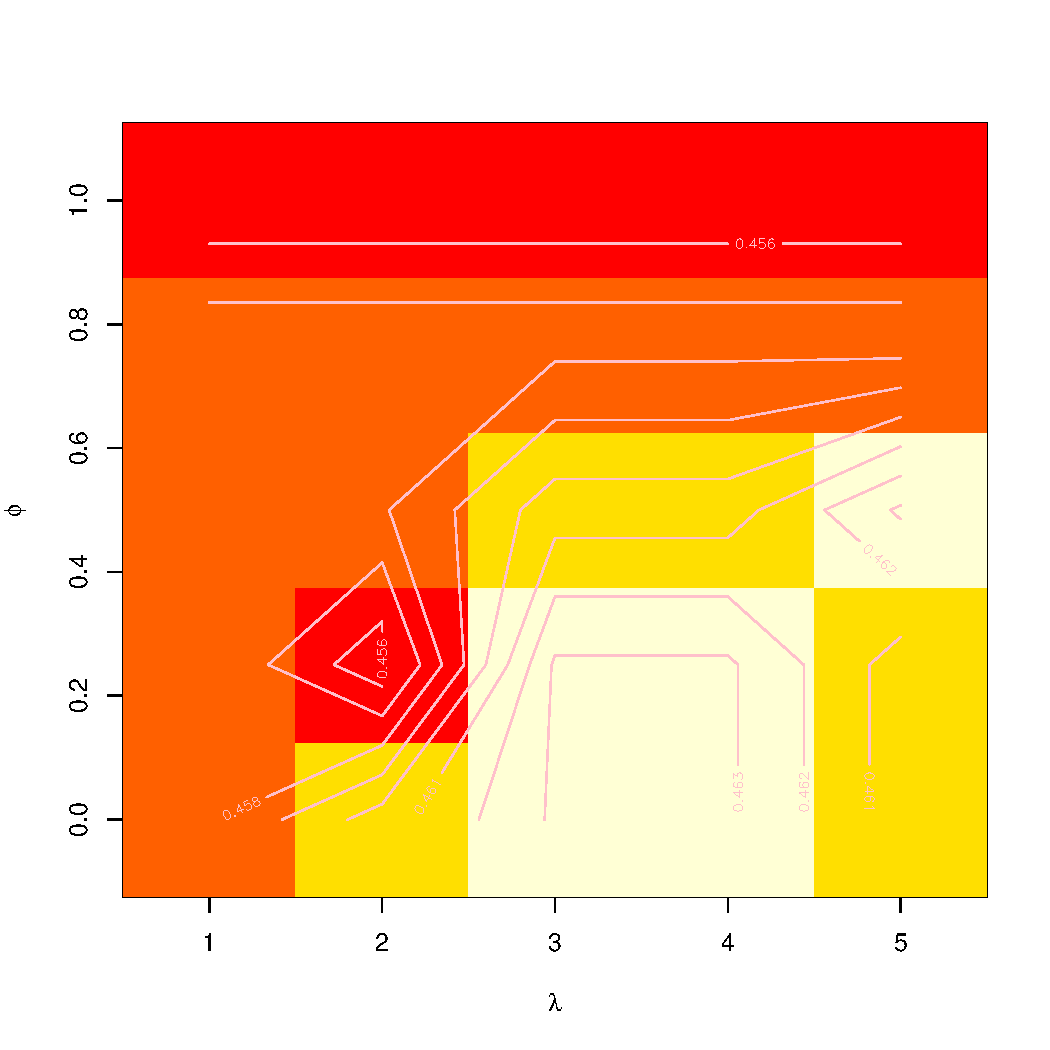
\includegraphics[width=5cm,height=4cm]{contour_dissimilaridade.pdf} }}%
    \caption[\scriptsize{Tunning parameters.}]{\scriptsize{ \textbf{(a)} Surface of parameters $\lambda$ and $k$ related with equation \ref{eq:vero}.\textbf{(b)}Contour of parameters $\lambda$ and $k$ related with equation \ref{eq:vero}.}}
    \label{fig:tunning}%
\end{figure}


O resultado para o modelo proposto não consegue identificar os resultados empate.

% latex table generated in R 3.3.2 by xtable 1.8-2 package
% Tue Nov 14 17:00:59 2017
\begin{table}[ht]
\centering
\begin{tabular}{crrrr}
  \hline
Seasons & Global & Home & Tie & Visitor \\ 
  \hline
2008-2014 & 47.11 & 79.65 & 0.00 & 36.52 \\ 
  2015 & 38.95 & 73.25 & 0.00 & 28.45 \\ 
  2016 & 56.32 & 85.56 & 0.00 & 49.54 \\ 
   \hline
\end{tabular}
    \caption[\scriptsize{Medidas do modelo.}]{\scriptsize{Medidas do modelo.}}
    \label{tab:medidasmod}
\end{table}


A tabela \ref{tab:forecastdissi} apresenta a simulação para o resultado da temporada de 2017/2018 baseada nos parâmetros estimados.


% latex table generated in R 3.3.2 by xtable 1.8-2 package
% Sun Nov 12 15:31:54 2017
\begin{table}[ht]
\centering
\begin{tabular}{lrrrr}
  \hline
Team & PLC & CCL& CEL & RET \\ 
  \hline
Man Utd & 16.50 & 49.02 & 14.96 & 1.77 \\ 
  Man City & 16.08 & 48.46 & 14.94 & 1.58 \\ 
  Tottenham & 12.90 & 43.01 & 15.79 & 1.98 \\ 
  Chelsea & 10.99 & 37.00 & 14.25 & 3.62 \\ 
  Arsenal & 9.32 & 35.04 & 14.77 & 3.83 \\ 
  Southampton & 8.70 & 36.16 & 14.13 & 3.08 \\ 
  Newcastle & 4.51 & 22.01 & 12.36 & 7.78 \\ 
  Crystal Palace & 3.85 & 19.93 & 11.86 & 9.30 \\ 
  Stoke City & 3.31 & 17.91 & 11.30 & 9.36 \\ 
  Everton & 2.79 & 16.15 & 10.55 & 11.90 \\ 
  Leicester & 1.85 & 10.63 & 8.78 & 16.67 \\ 
  Liverpool & 1.77 & 12.71 & 8.93 & 14.09 \\ 
  Watford & 1.69 & 9.36 & 7.82 & 16.87 \\ 
  West Brom & 1.52 & 10.38 & 8.18 & 17.85 \\ 
  Bournemouth & 1.52 & 8.61 & 7.53 & 19.35 \\ 
  Swansea & 1.14 & 8.78 & 7.97 & 19.50 \\ 
  Burnley & 0.60 & 4.68 & 5.03 & 29.40 \\ 
  West Ham & 0.46 & 4.25 & 4.81 & 31.67 \\ 
  Brighton & 0.40 & 4.31 & 4.06 & 32.00 \\ 
  Huddersfield & 0.10 & 1.62 & 1.98 & 48.40 \\ 
   \hline
\end{tabular}
    \caption[\scriptsize{TAVB}]{\scriptsize{Detailed table of competition where the values are probability of the simulation. Premier League Champion (PLC), Classify to UEFA Champions League (CCL), Classify to UEFA Europa League (CEL) Relegated team (RE).}}
    \label{tab:forecastdissi}
\end{table}



Isso ocorre devido o valor de $X_r$ representar uma medida de \textbf{dissimilaridade}, isto é, quanto maior o valor $X_r$ mais diferente são as habilidades do time mandante e visitante. Caso as habilidades dos dois times sejam iguais o valor  $X_r$ zera, inviabilizando a regressão do parâmetro $\alpha_{Tie}$. 

Dessa forma, propomos uma medida de \textbf{similaridade} para regressão do parâmetro $\alpha_{Tie}$ relativo ao empate. Faremos:

\begin{equation}
X_r^{Tie} = \gamma \exp{\left\{-\sigma X_r ^2\right\}}
\end{equation}

Nessa estratégia, os parâmetros $\lambda$, $\phi$, $\sigma$ e $\gamma$ são determinados utilizando a procedimento \textit{tuning}. O modelo para $\alpha_{Tie}$ captará o nível de similaridade dos times.


% latex table generated in R 3.3.2 by xtable 1.8-2 package
% Tue Nov 14 19:42:00 2017
\begin{table}[ht]
\centering
\begin{tabular}{cc|r|rrr}
  \hline
Seasons & Data & \textbf{Global} & Home & Tie & Visitor \\ 
  \hline
2008-2014 & Trainning & 56.97 & 80.91 & 8.77 & 56.30 \\ 
  2015 & Tuning & 44.21 & 71.34 & 3.74 & 44.83 \\ 
  2016 & Test & 51.05 & 66.84 & 4.76 & 59.63 \\ 
   \hline
\end{tabular}
    \caption[\scriptsize{Medidas do modelo com similaridade para o empate.}]{\scriptsize{Medidas do modelo que inclue o ajuste para similaridade do empate.}}
    \label{tab:medidasmodsi}
\end{table}	



% latex table generated in R 3.3.2 by xtable 1.8-2 package
% Sun Nov 12 15:31:54 2017
\begin{table}[ht]
\centering
\begin{tabular}{lrrrr}
  \hline
Team & PLC & CCL& CEL & RET \\ 
  \hline
  Liverpool & 39.00 & 86.00 & 7.00 & 0.00 \\ 
  Man City & 31.00 & 78.00 & 12.00 & 0.00 \\ 
  Chelsea & 13.00 & 62.00 & 17.00 & 0.00 \\ 
  Leicester & 6.00 & 34.00 & 24.00 & 0.00 \\ 
  Tottenham & 5.00 & 32.00 & 24.00 & 2.00 \\ 
  Man Utd & 4.00 & 26.00 & 19.00 & 0.00 \\ 
  Stoke City & 1.00 & 26.00 & 26.00 & 0.00 \\ 
  Everton & 1.00 & 14.00 & 8.00 & 3.00 \\ 
  West Ham & 0.00 & 9.00 & 13.00 & 10.00 \\ 
  West Brom & 0.00 & 11.00 & 17.00 & 4.00 \\ 
  Watford & 0.00 & 0.00 & 3.00 & 21.00 \\ 
  Swansea & 0.00 & 1.00 & 5.00 & 17.00 \\ 
  Southampton & 0.00 & 6.00 & 6.00 & 16.00 \\ 
  Newcastle & 0.00 & 3.00 & 3.00 & 9.00 \\ 
  Huddersfield & 0.00 & 0.00 & 0.00 & 64.00 \\ 
  Crystal Palace & 0.00 & 1.00 & 5.00 & 21.00 \\ 
  Burnley & 0.00 & 0.00 & 0.00 & 84.00 \\ 
  Brighton & 0.00 & 2.00 & 1.00 & 18.00 \\ 
  Bournemouth & 0.00 & 0.00 & 1.00 & 27.00 \\ 
  Arsenal & 0.00 & 9.00 & 9.00 & 4.00 \\ 
   \hline
\end{tabular}
    \caption[\scriptsize{TAVB} with similarity]{\scriptsize{Detailed table of competition where the values are probability of the simulation with similarity for tie. Premier League Champion (PLC), Classify to UEFA Champions League (CCL), Classify to UEFA Europa League (CEL) Relegated team (RE).}}
    \label{tab:forecastsi}
\end{table}

Apesar de pequena, o tratamento para a regressão do coeficiente do emapate contribui para melhorar o poder de previsibilidade do modelo.


\section{Resultados}
\label{sec:reslt}

\newpage

\begin{figure}
\begin{tabular}{ccccc}
  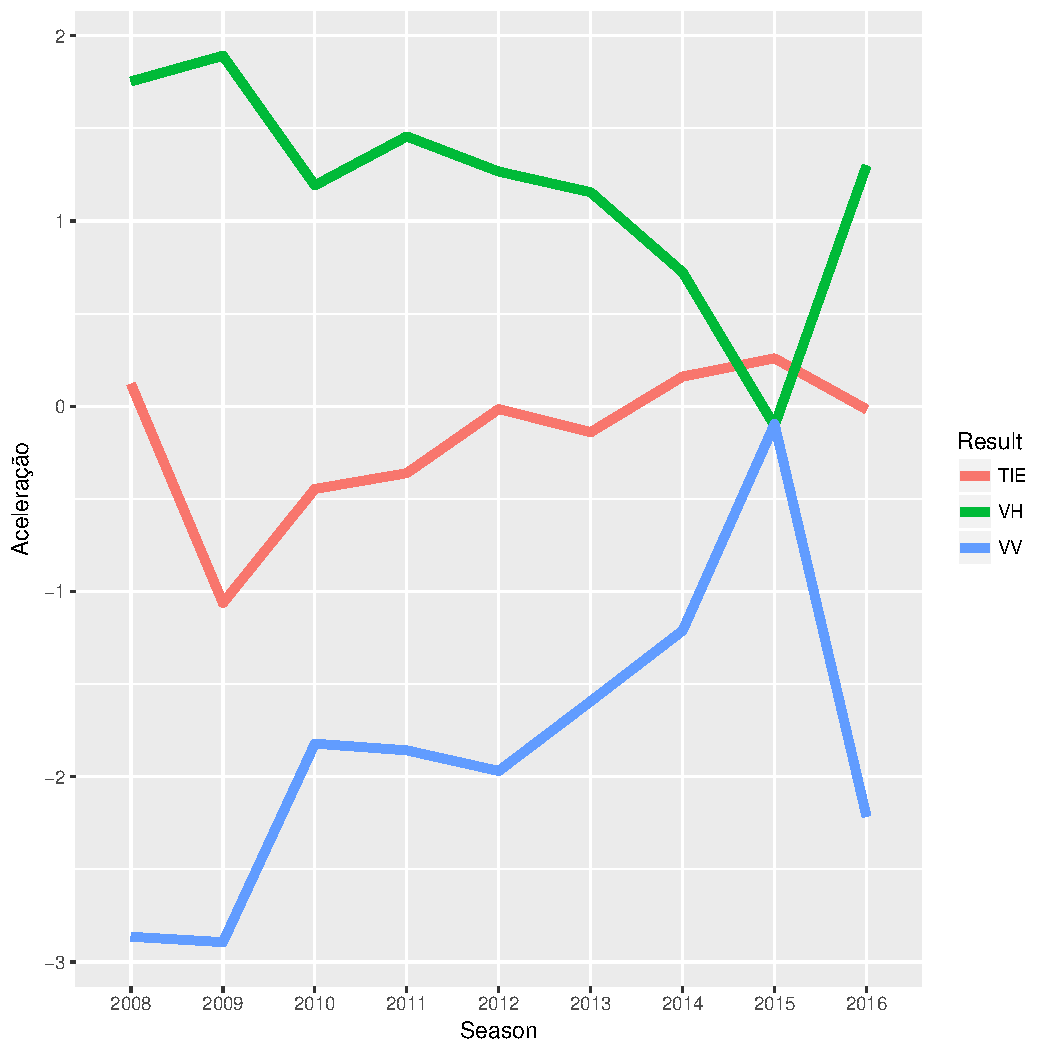
\includegraphics[width=25mm]{aceleracao_result} & 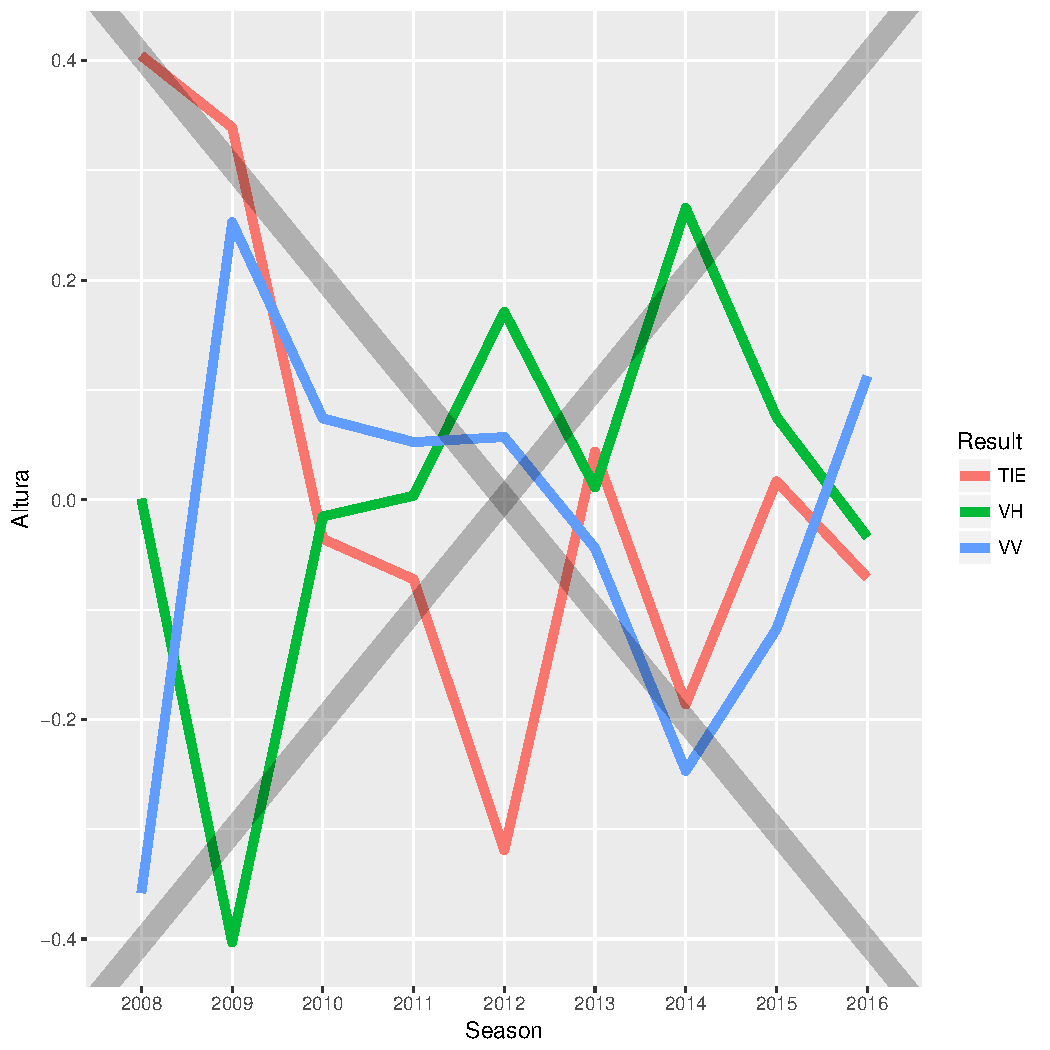
\includegraphics[width=25mm]{altura_result} & 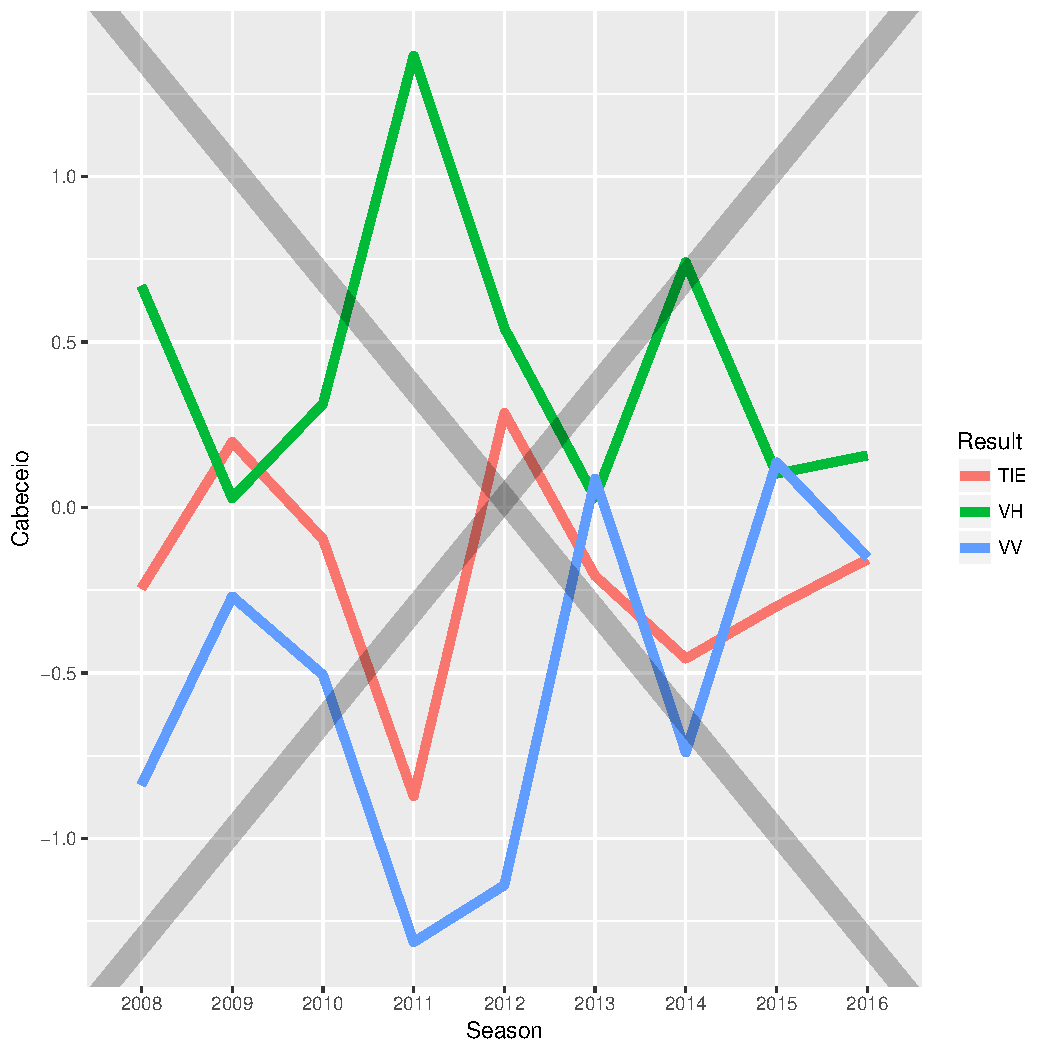
\includegraphics[width=25mm]{cabeceio_result} &   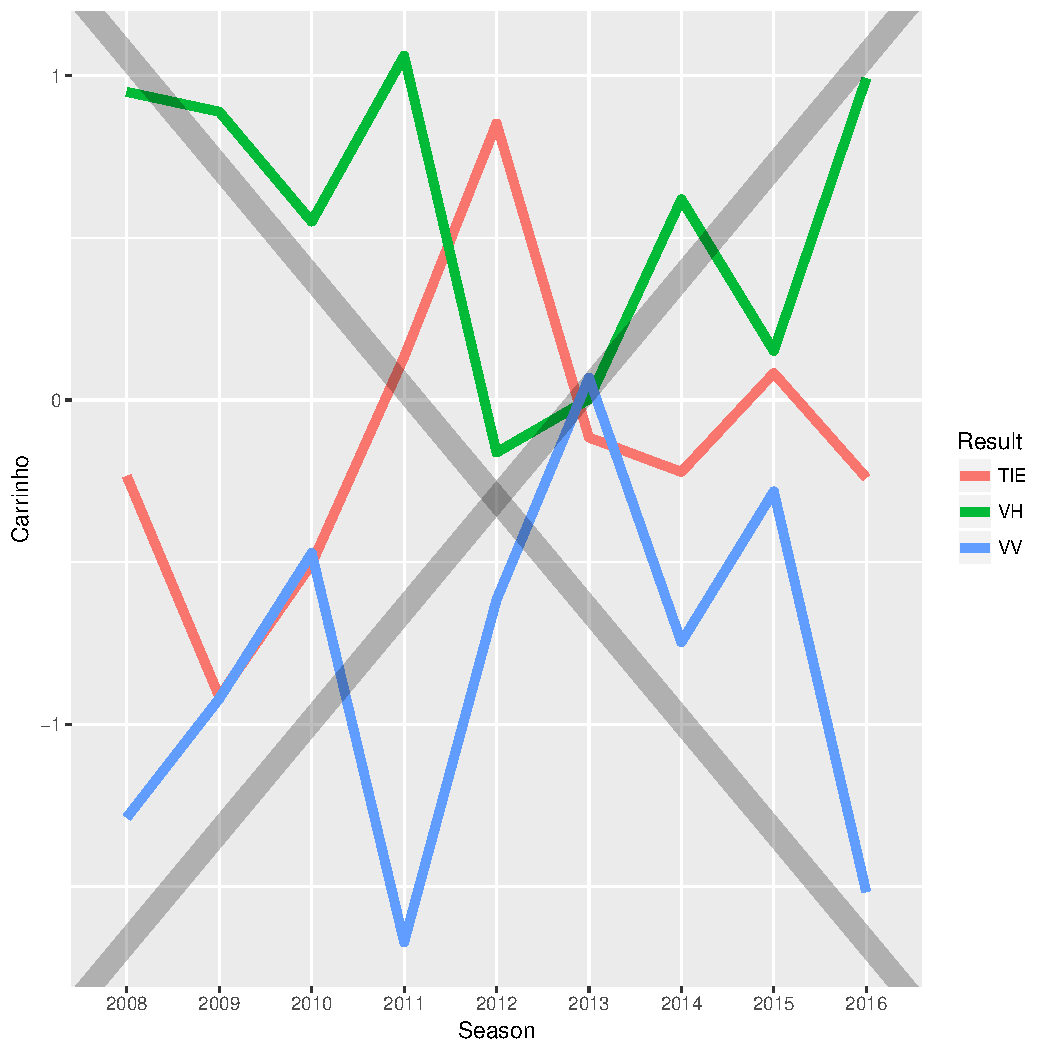
\includegraphics[width=25mm]{carrinho_result} &
  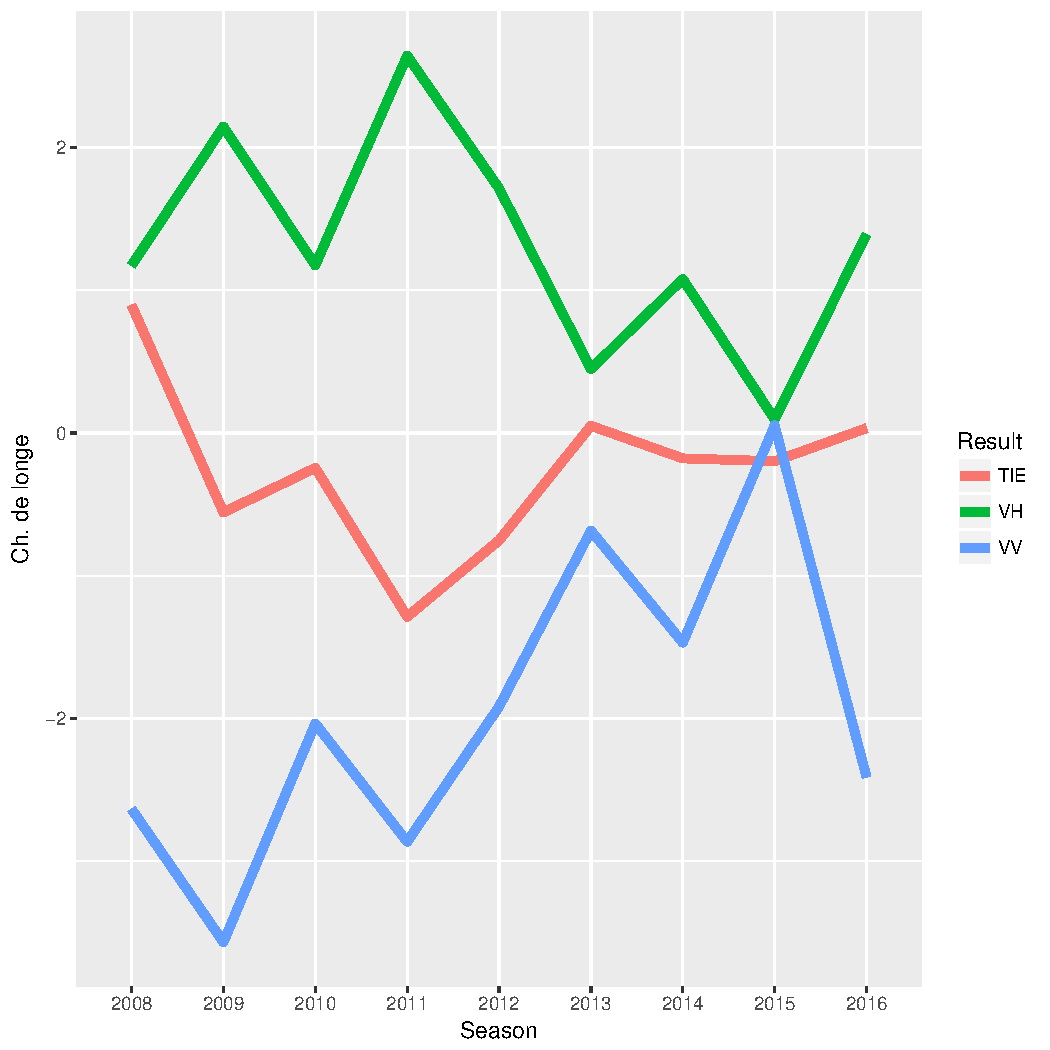
\includegraphics[width=25mm]{ch_delonge_result} \\
\scriptsize{(a) Aceleração } & \scriptsize{(b) altura  } & \scriptsize{(c) cabeceio } & \scriptsize{(d) carrinho } & \scriptsize{(e) chute de longe }\\[3pt]
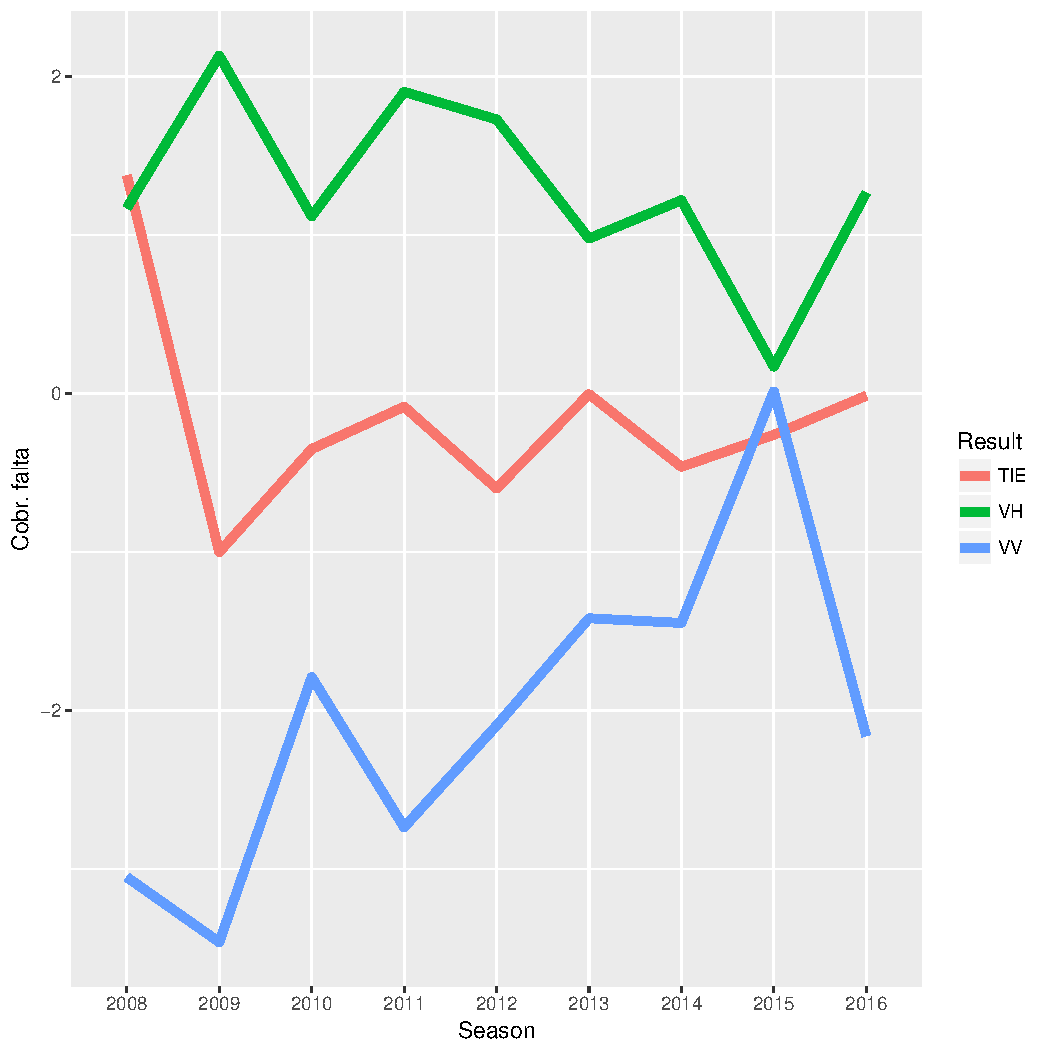
\includegraphics[width=25mm]{cobr_falta_result} & 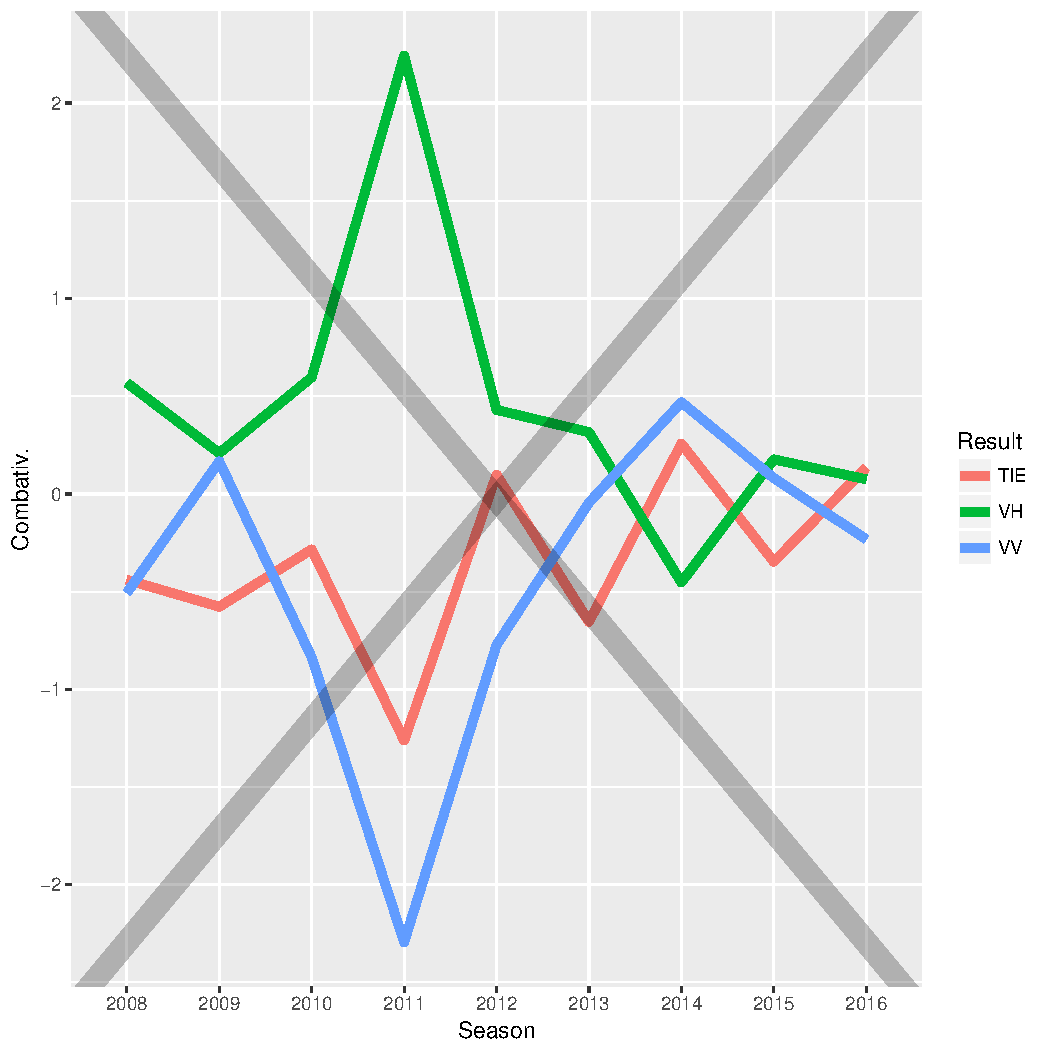
\includegraphics[width=25mm]{combativ__result} &   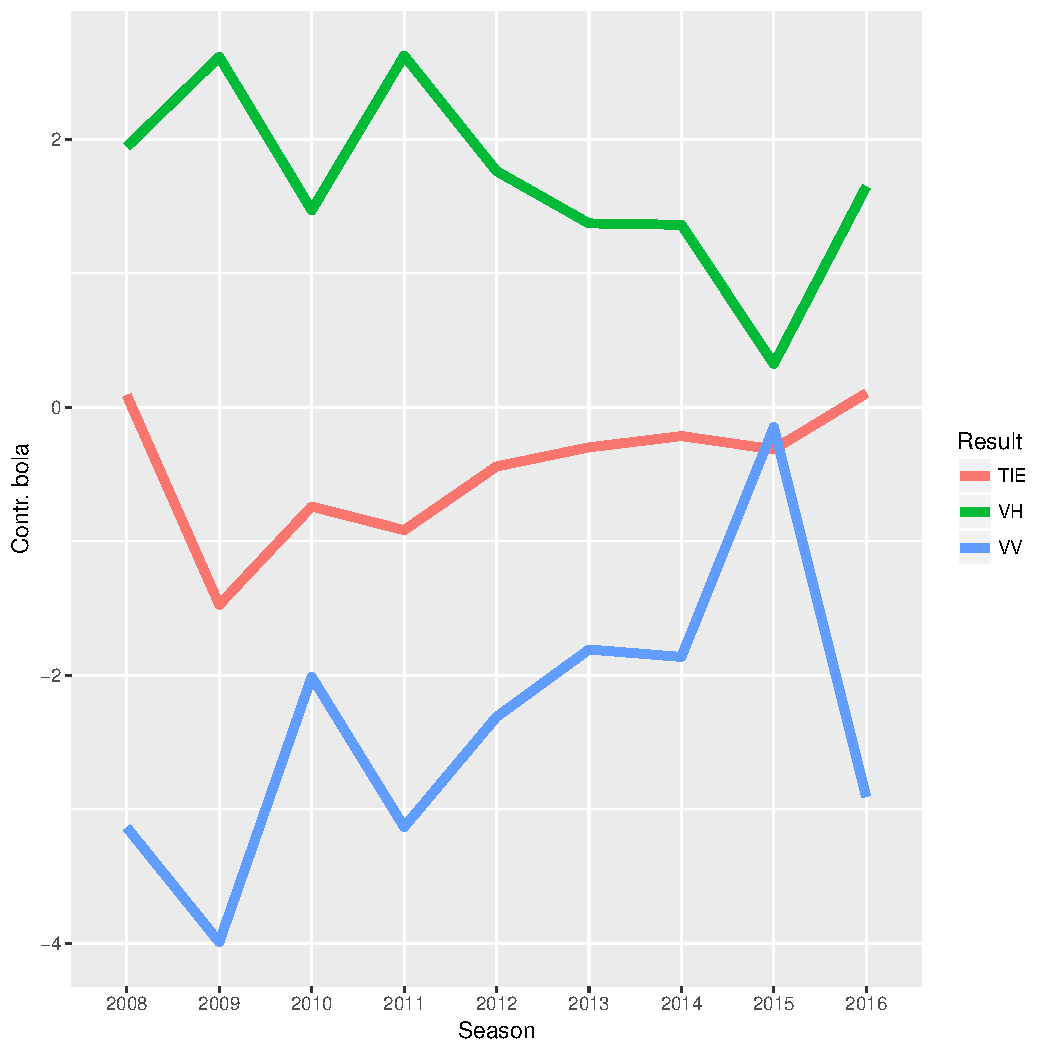
\includegraphics[width=25mm]{contr_bola_result} &
  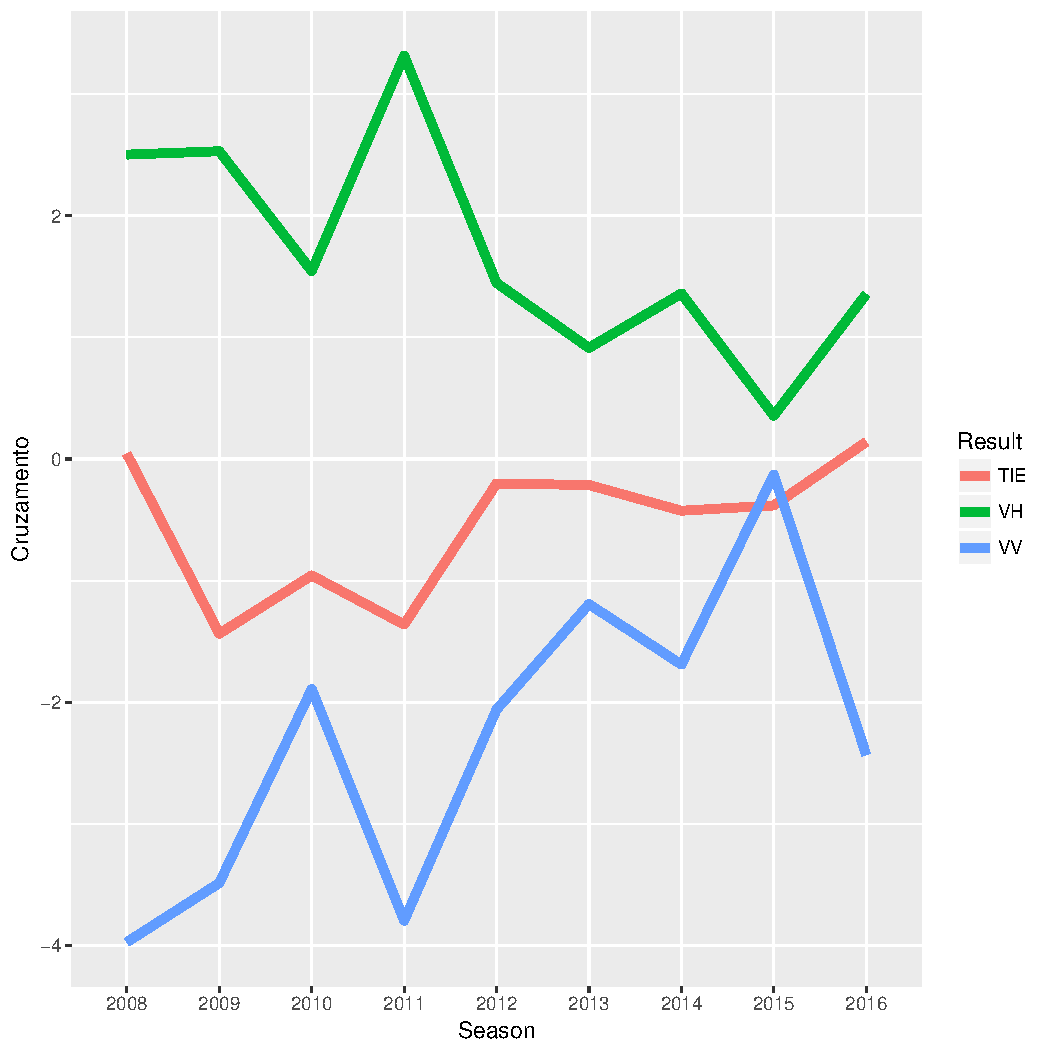
\includegraphics[width=25mm]{cruzamento_result} & 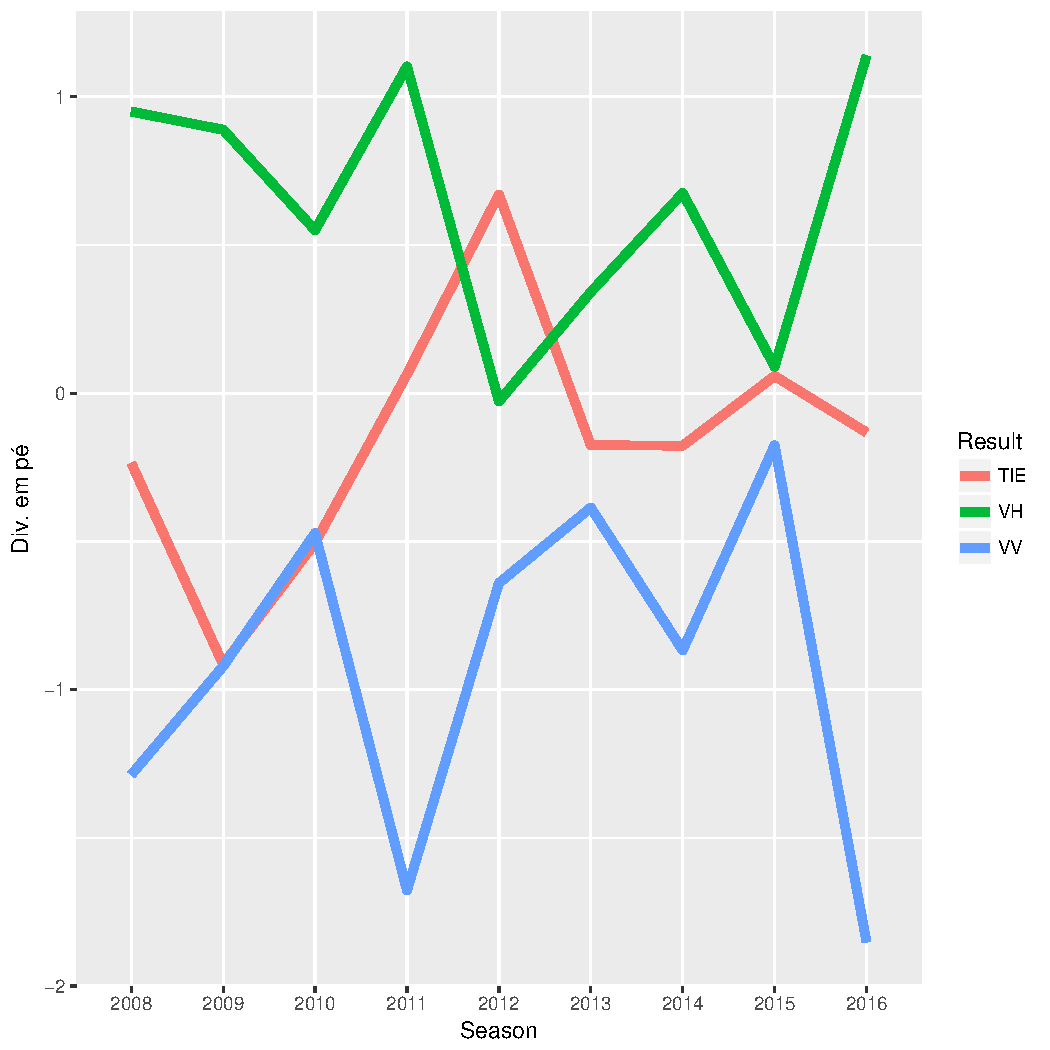
\includegraphics[width=25mm]{div_empe_result} \\
 \scriptsize{(f) cobrança de falta } & \scriptsize{(g) combatividade } & \scriptsize{(h) controle de bola} & \scriptsize{(i) cruzamento} & \scriptsize{(j) dividida}\\[3pt]
 
 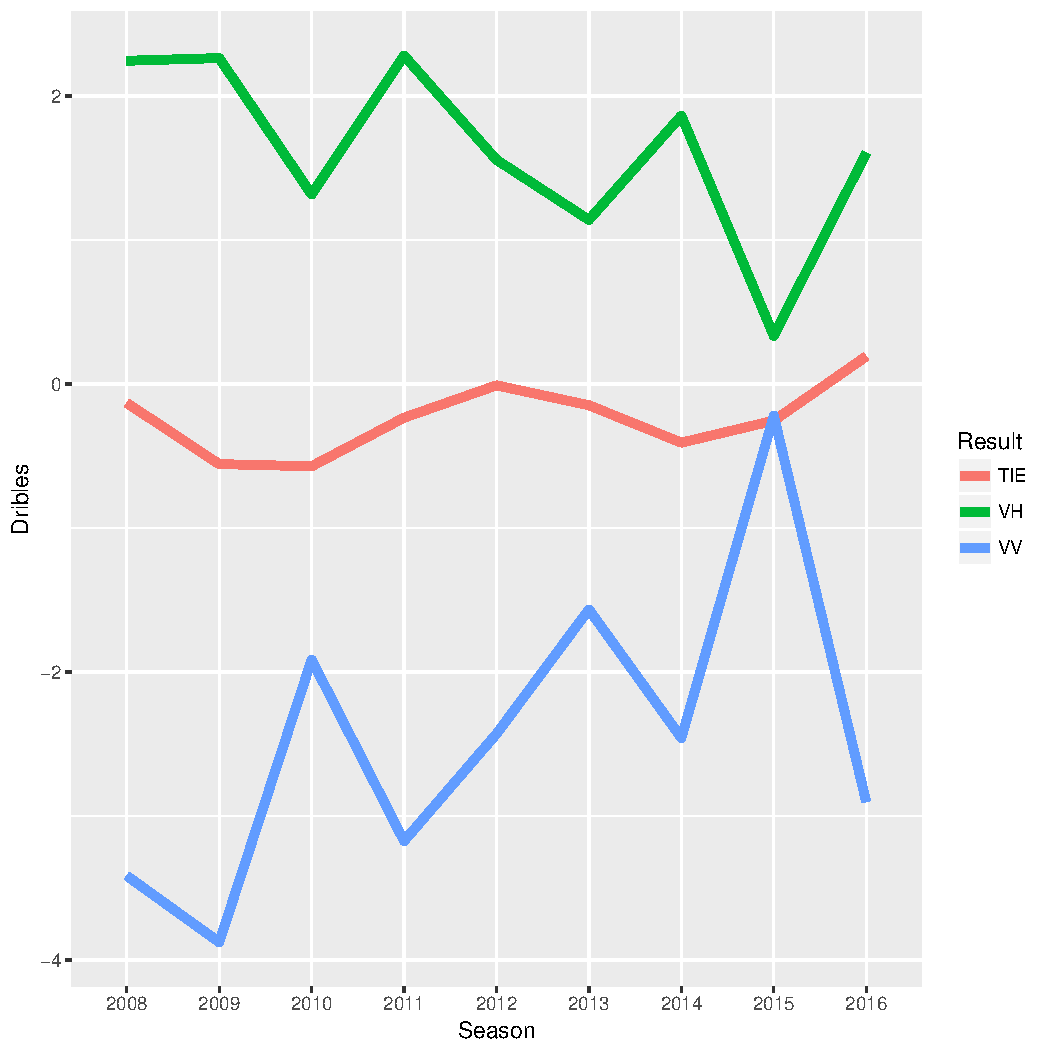
\includegraphics[width=25mm]{dribles_result} & 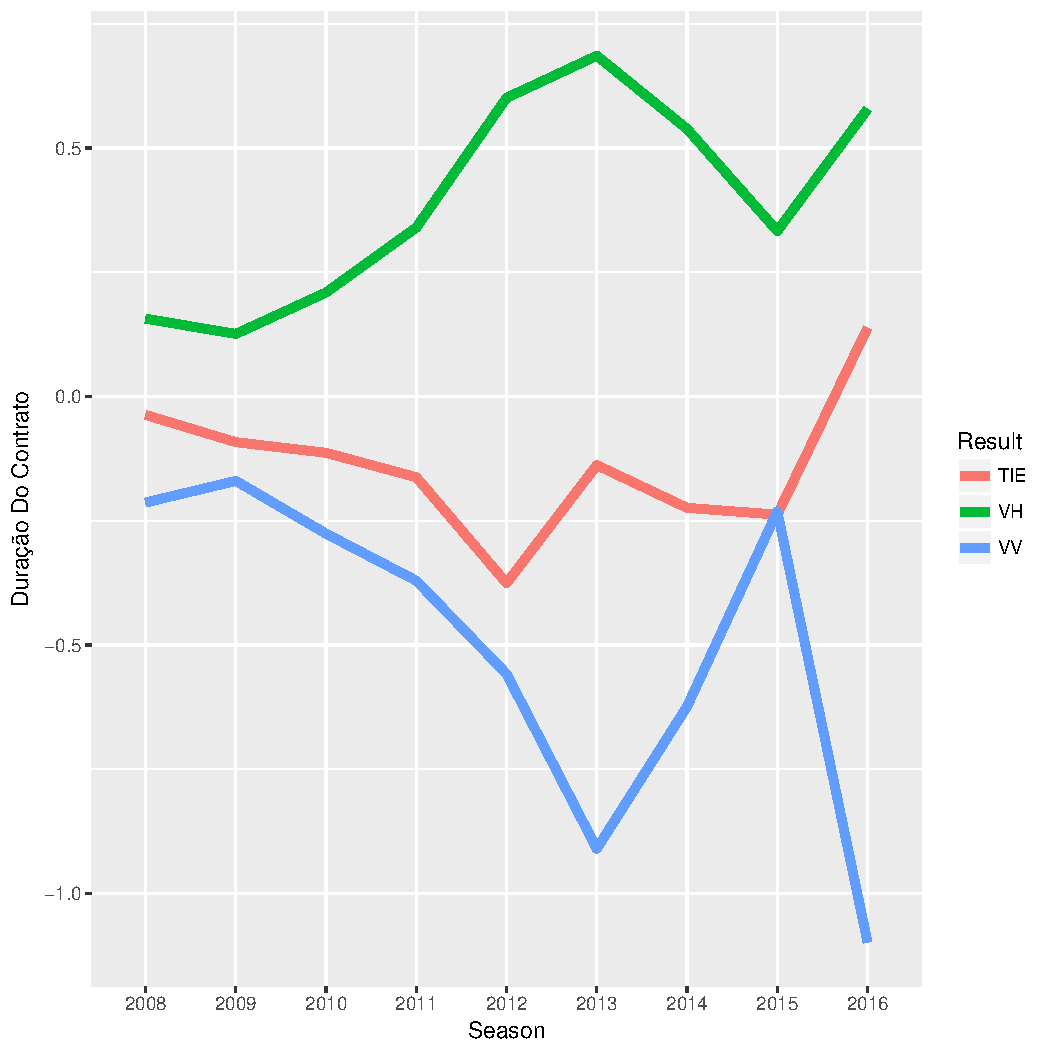
\includegraphics[width=25mm]{duracaodocontrato_result} &   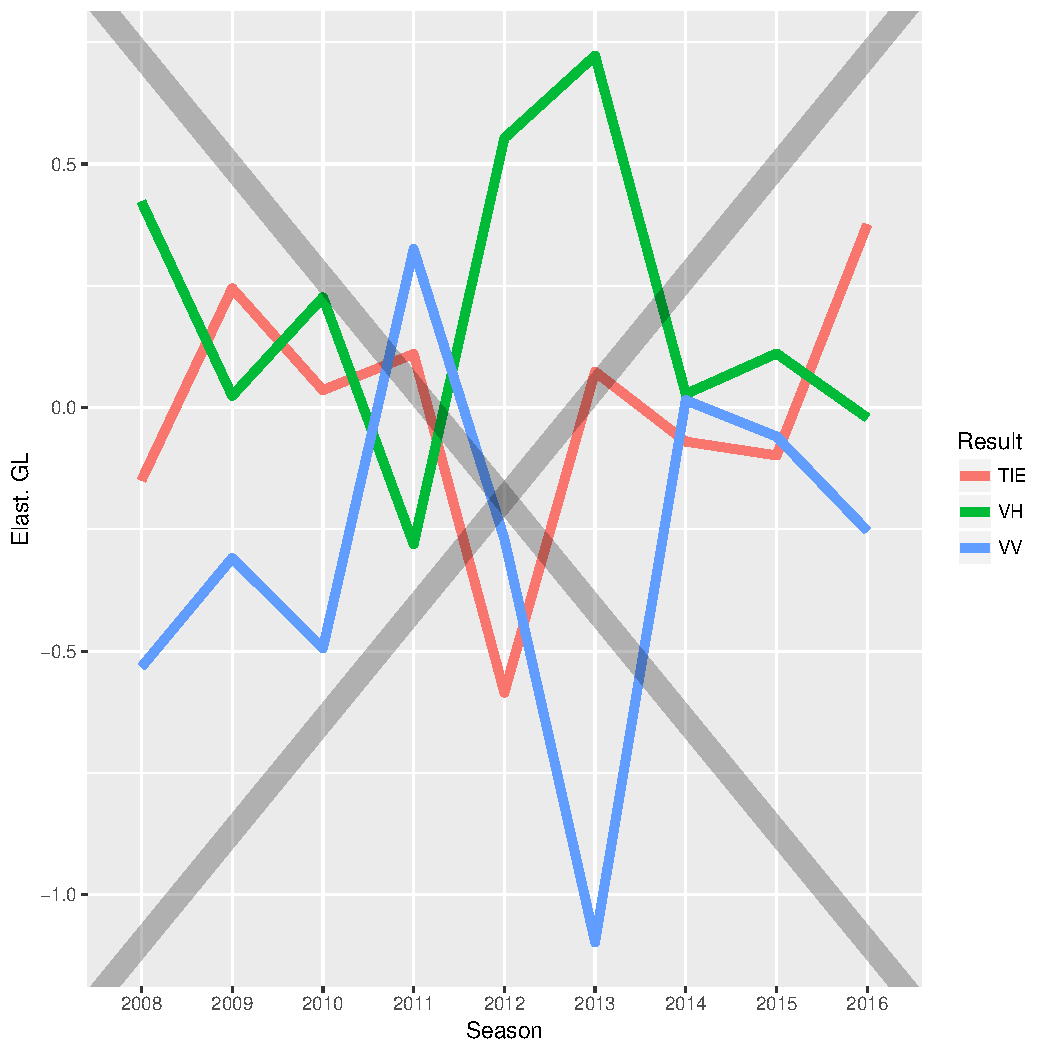
\includegraphics[width=25mm]{elast_gl_result} &
  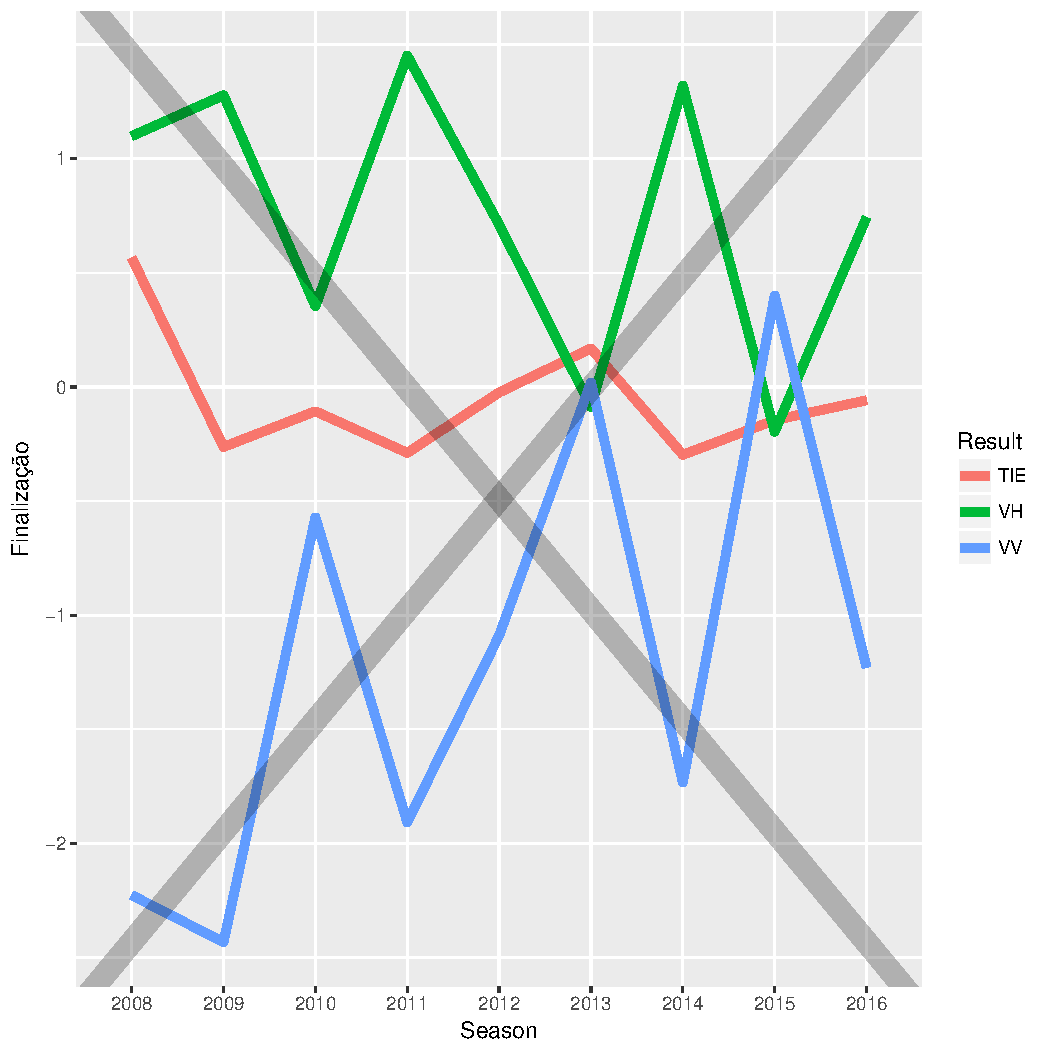
\includegraphics[width=25mm]{finalizacao_result} & 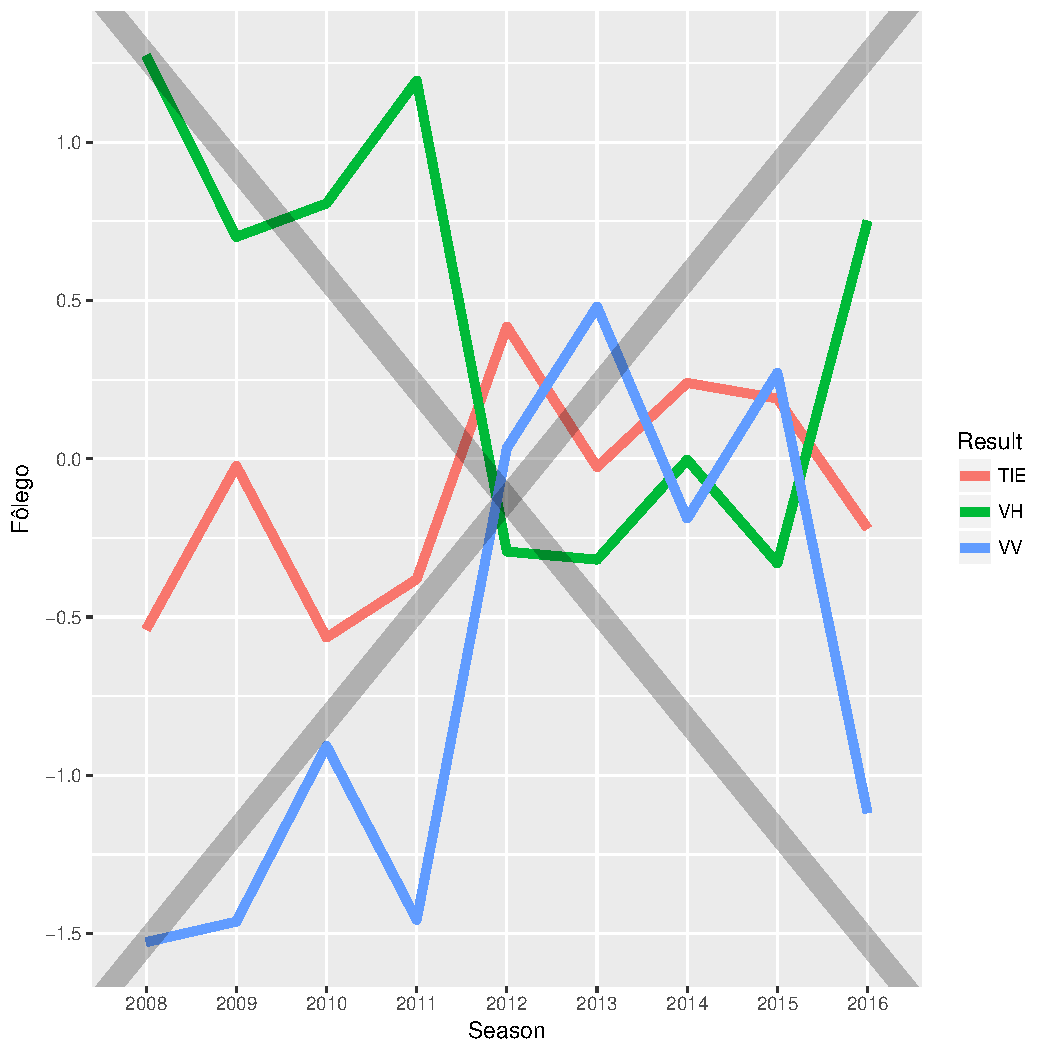
\includegraphics[width=25mm]{folego_result}  \\
 \scriptsize{(k) drible} & \scriptsize{(l) duração do contrato } & \scriptsize{(m) elasticidade do goleiro} & \scriptsize{(n) finalização} & \scriptsize{(o) fôlego}\\[3pt]
 
  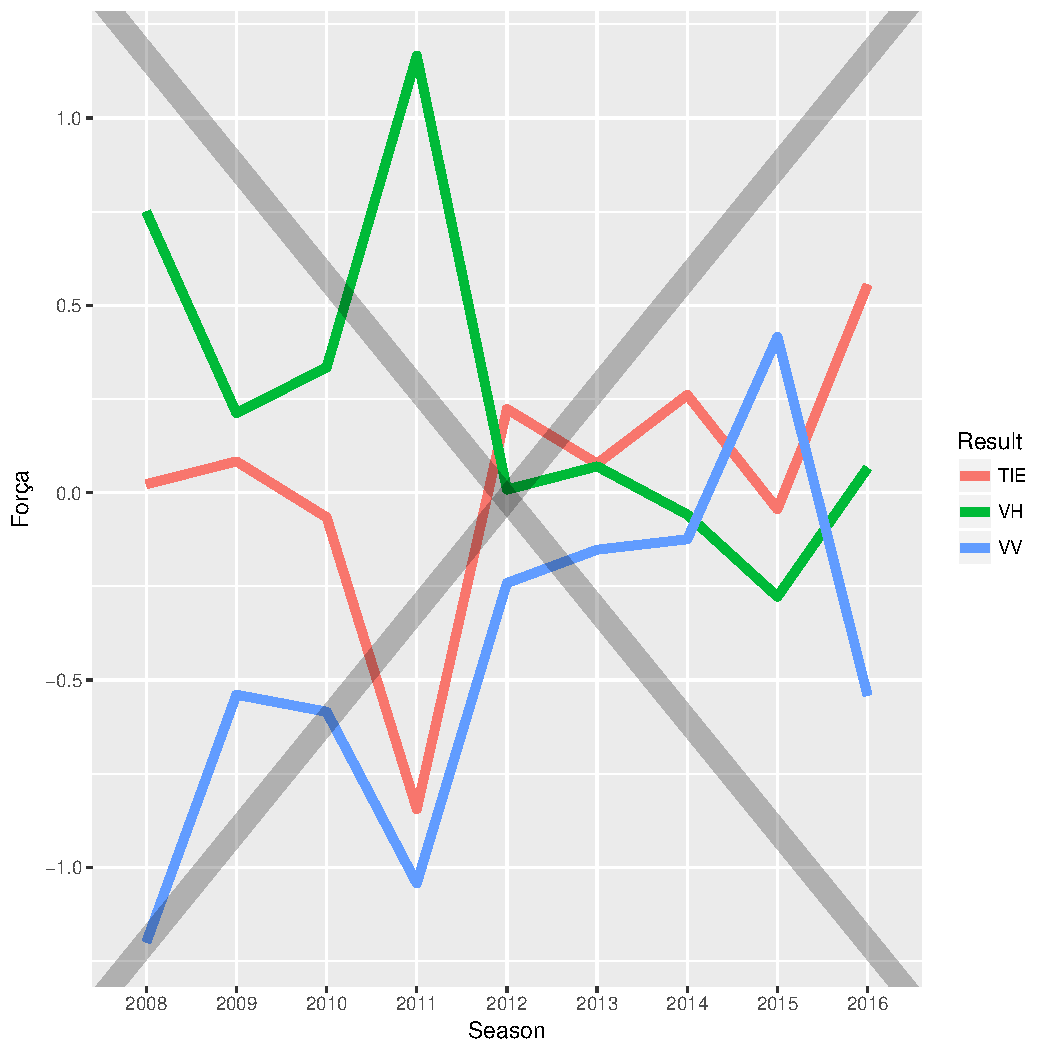
\includegraphics[width=25mm]{forca_result} & 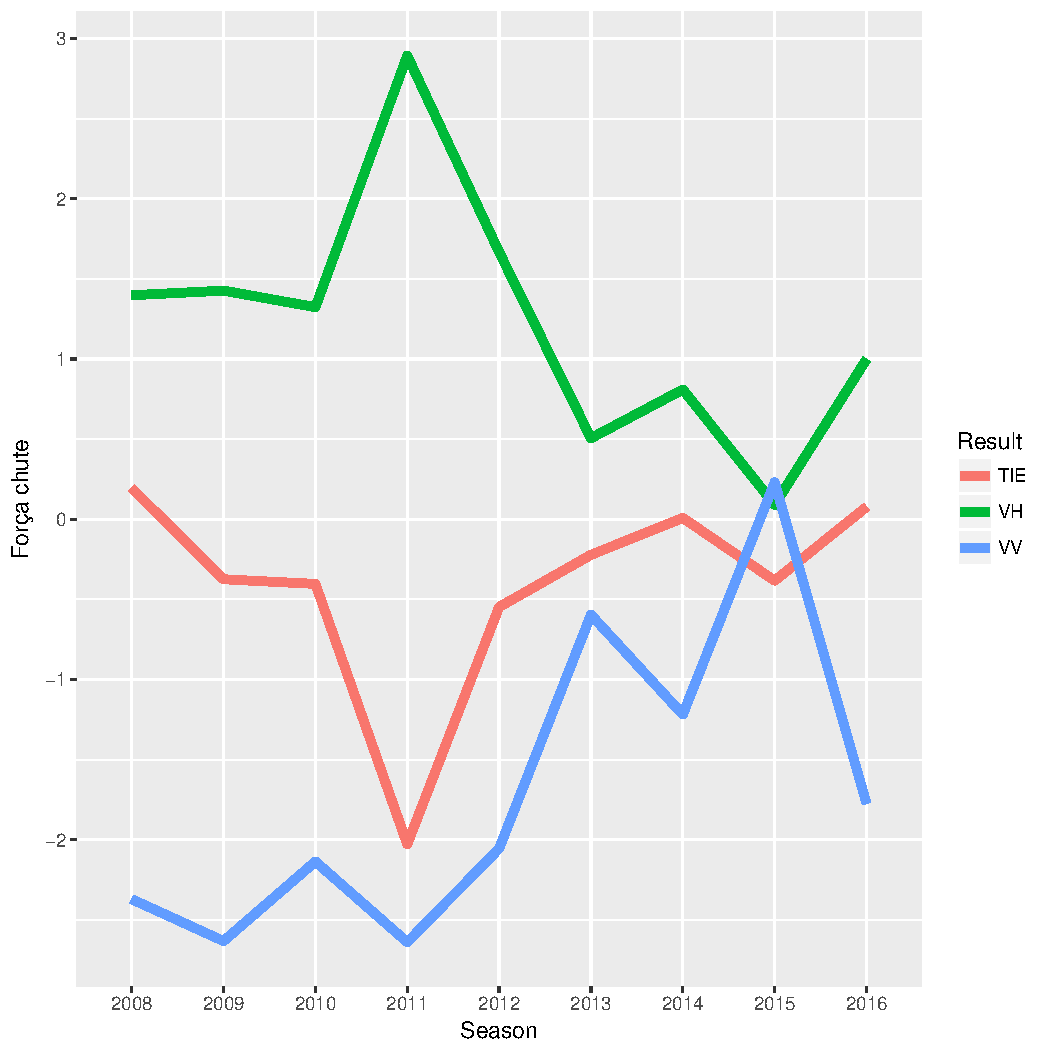
\includegraphics[width=25mm]{forcachute_result}  &   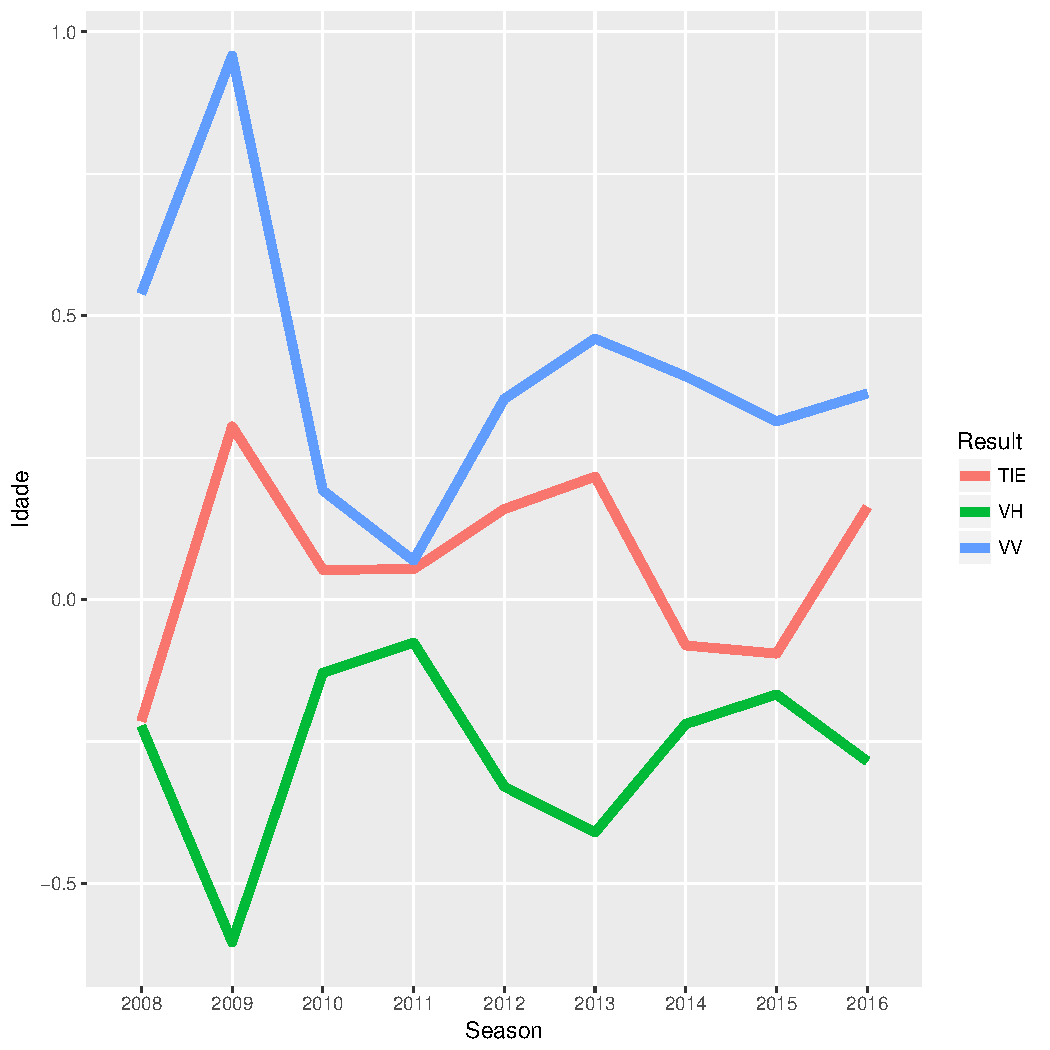
\includegraphics[width=25mm]{idade_result} &
  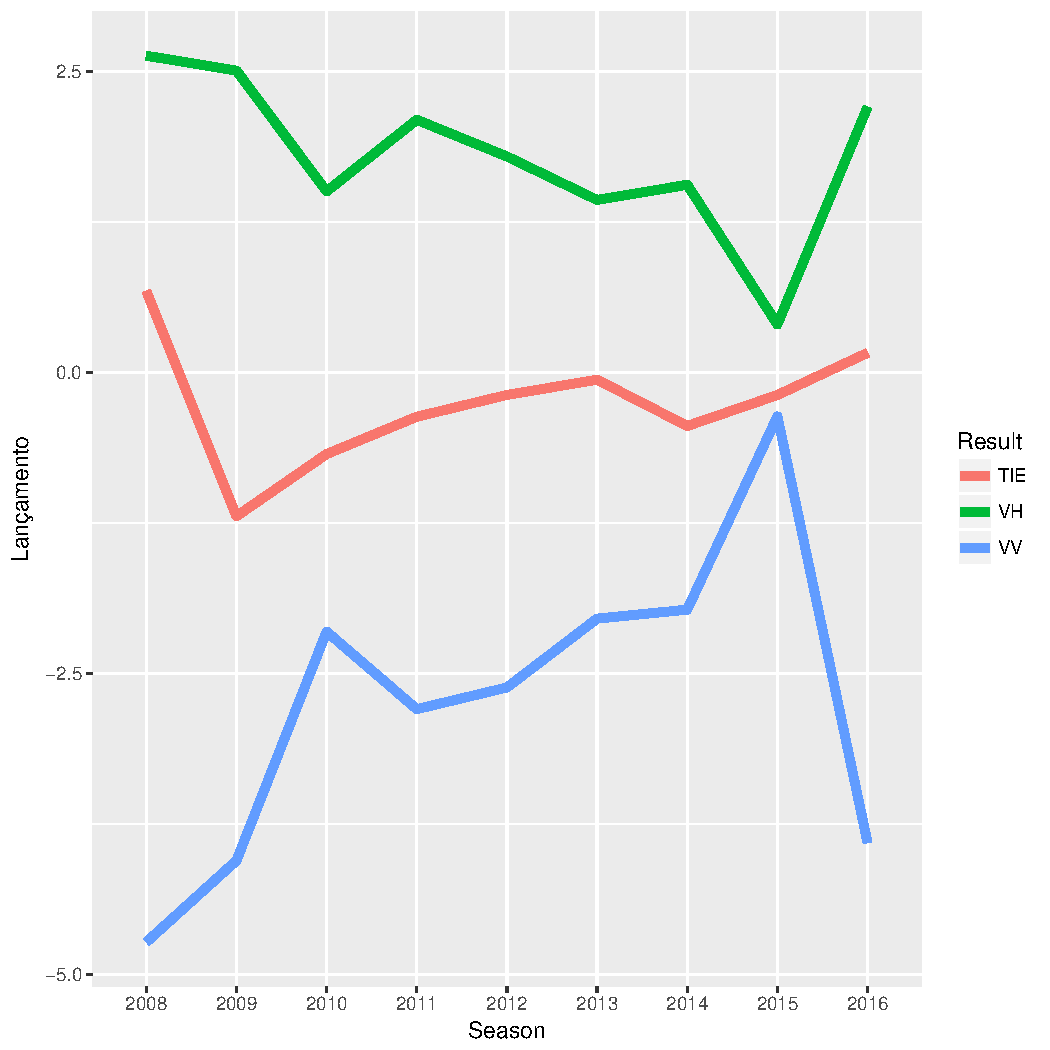
\includegraphics[width=25mm]{lancamento_result}  & 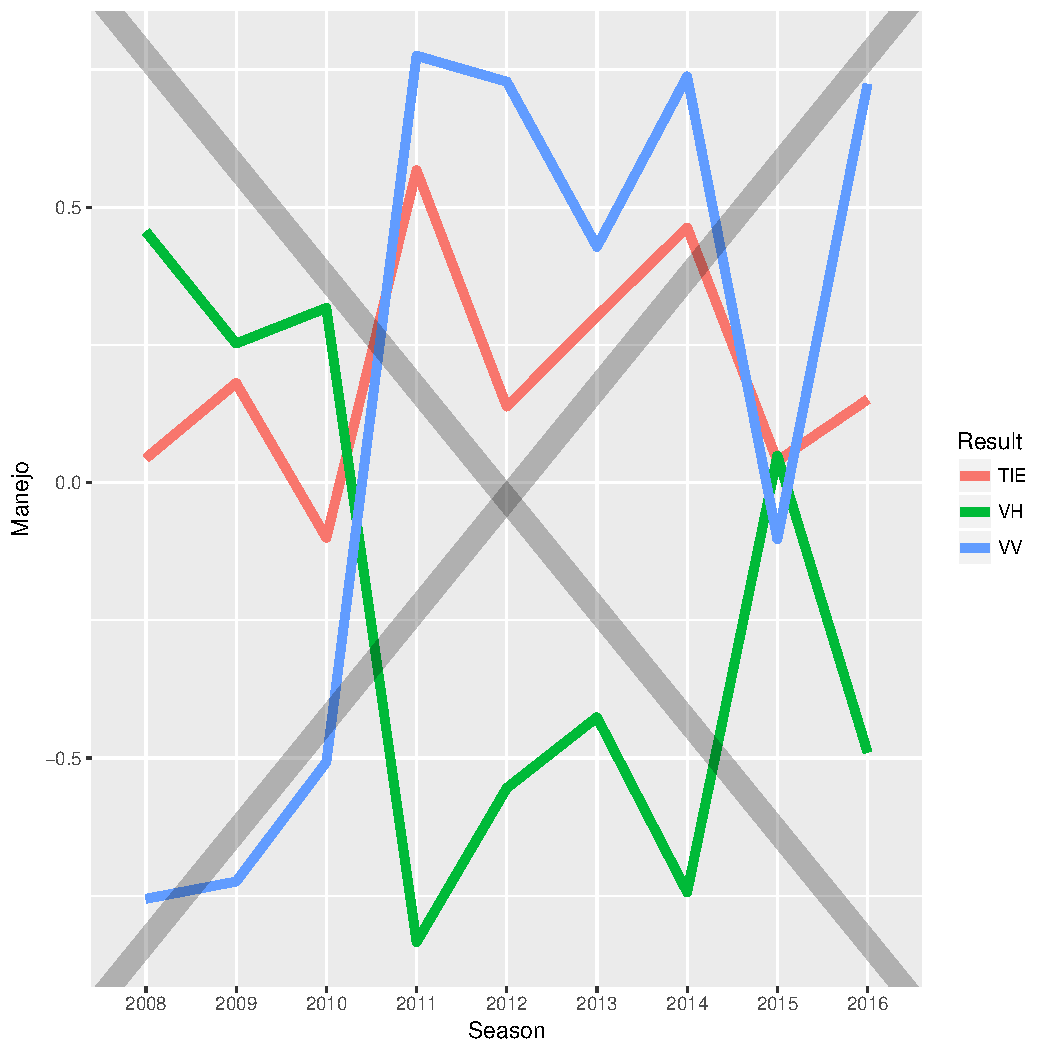
\includegraphics[width=25mm]{manejo_result}  \\
 \scriptsize{(p) força} & \scriptsize{(q) força chute } & \scriptsize{(r) idade} & \scriptsize{(s) lançamento} & \scriptsize{(t) manejo}\\[3pt]
 
   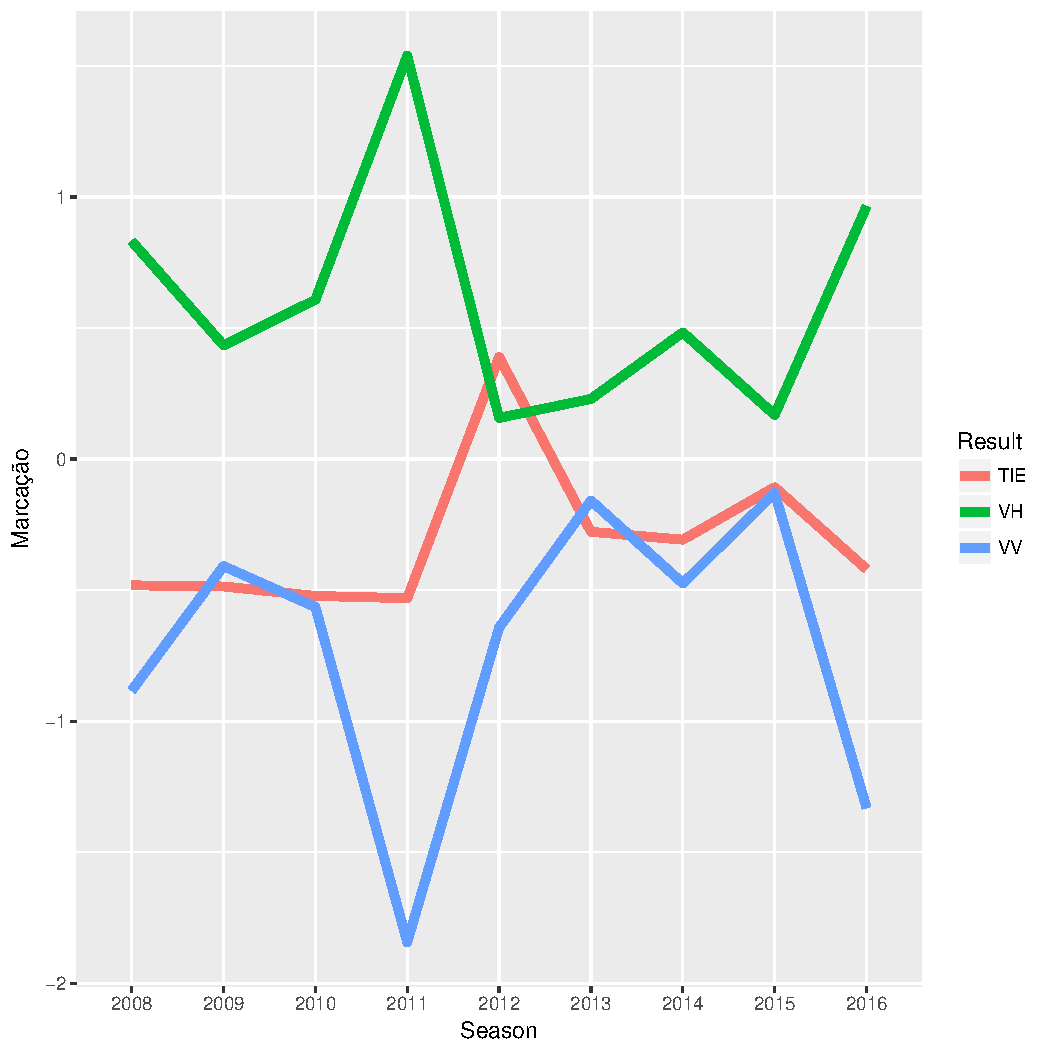
\includegraphics[width=25mm]{marcacao_result} & 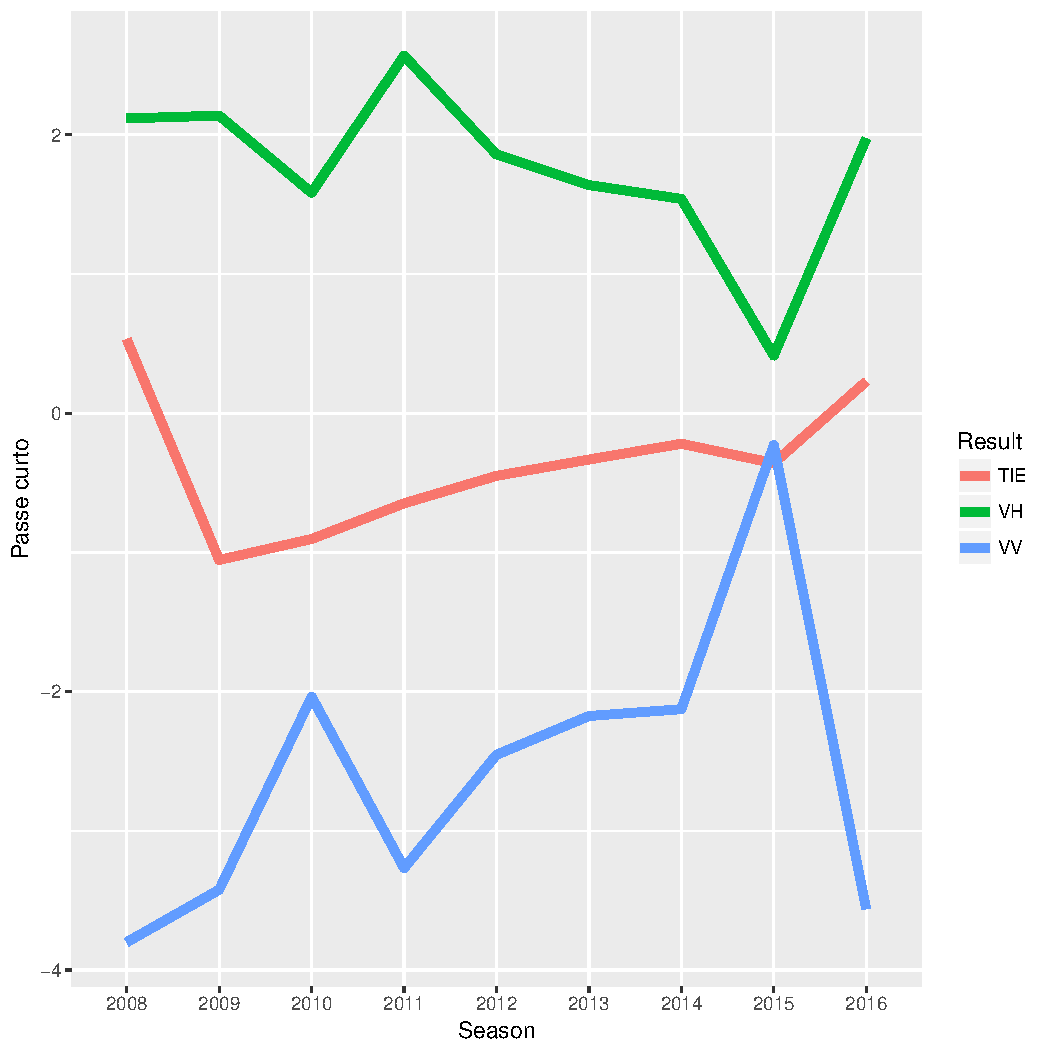
\includegraphics[width=25mm]{passecurto_result}   &   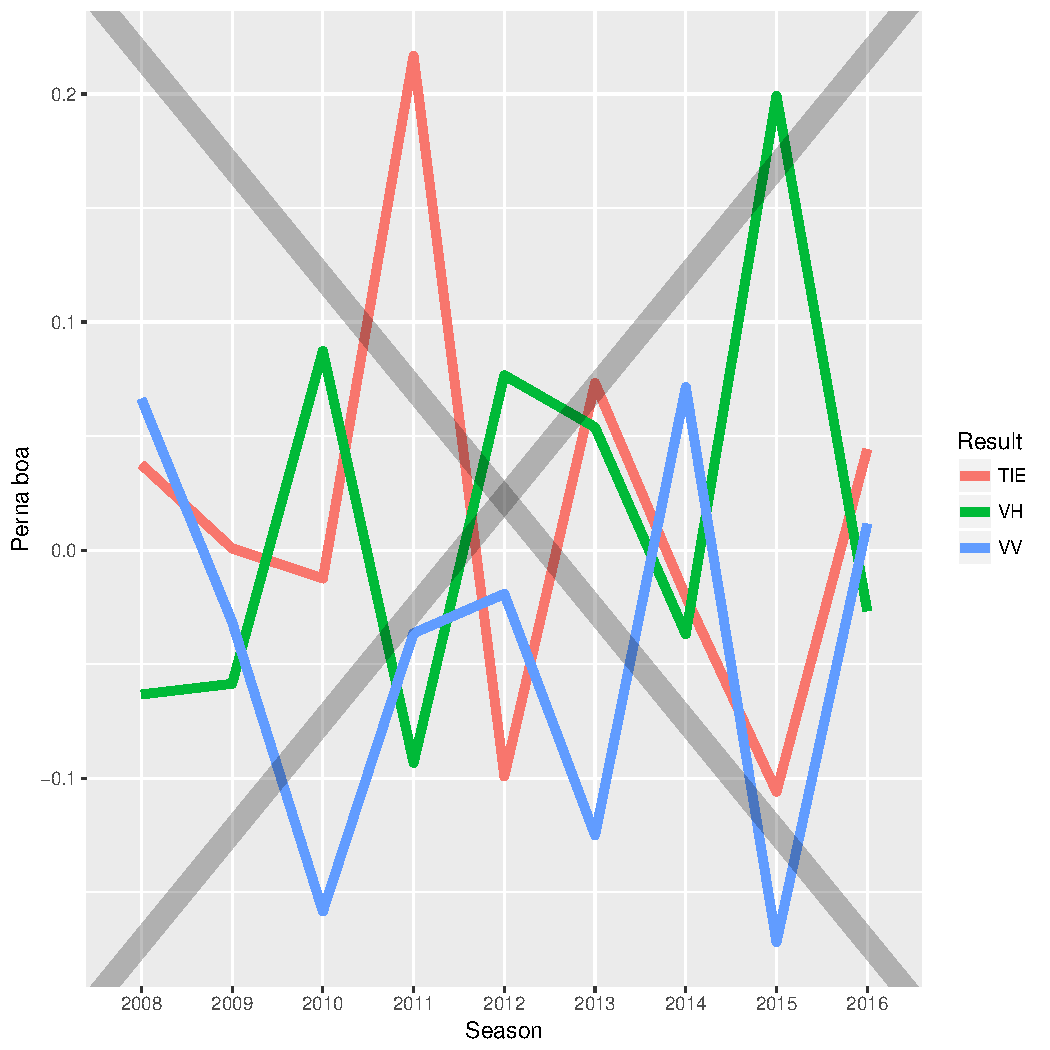
\includegraphics[width=25mm]{pernaboa_result}&
  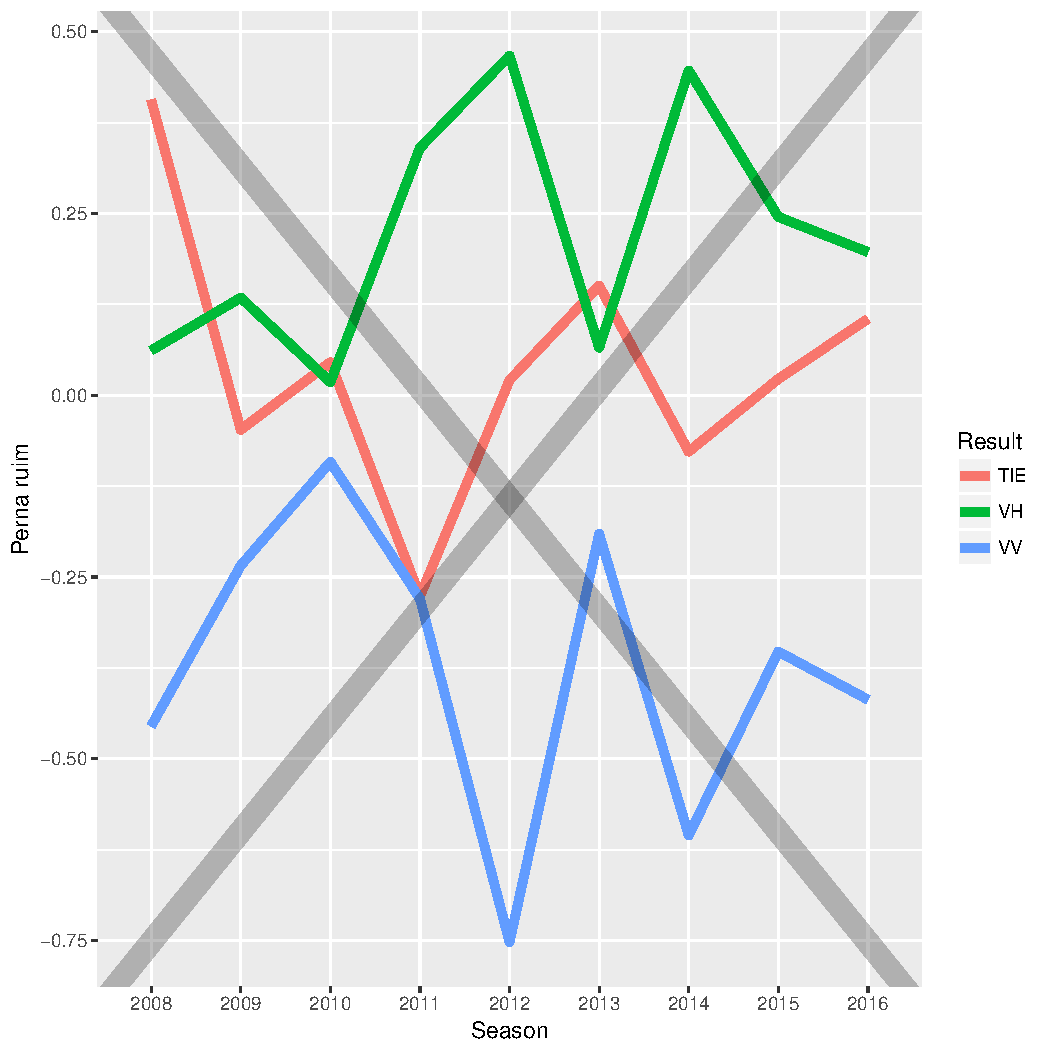
\includegraphics[width=25mm]{pernaruim_result}   & 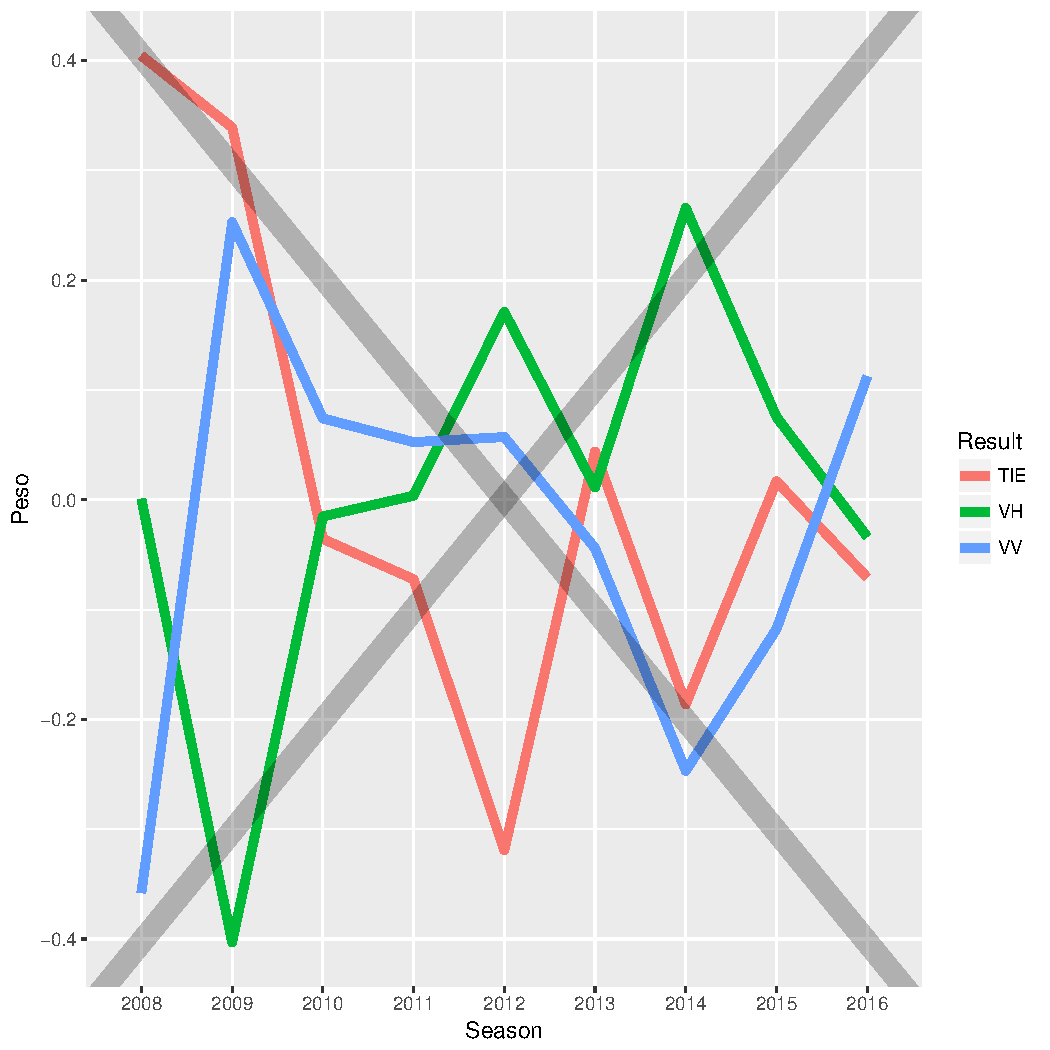
\includegraphics[width=25mm]{peso_result}   \\
 \scriptsize{(u) marcação} & \scriptsize{(v) passe curto } & \scriptsize{(w) perna boa} & \scriptsize{(x) perna ruim} & \scriptsize{(y) peso}\\[3pt]
 
    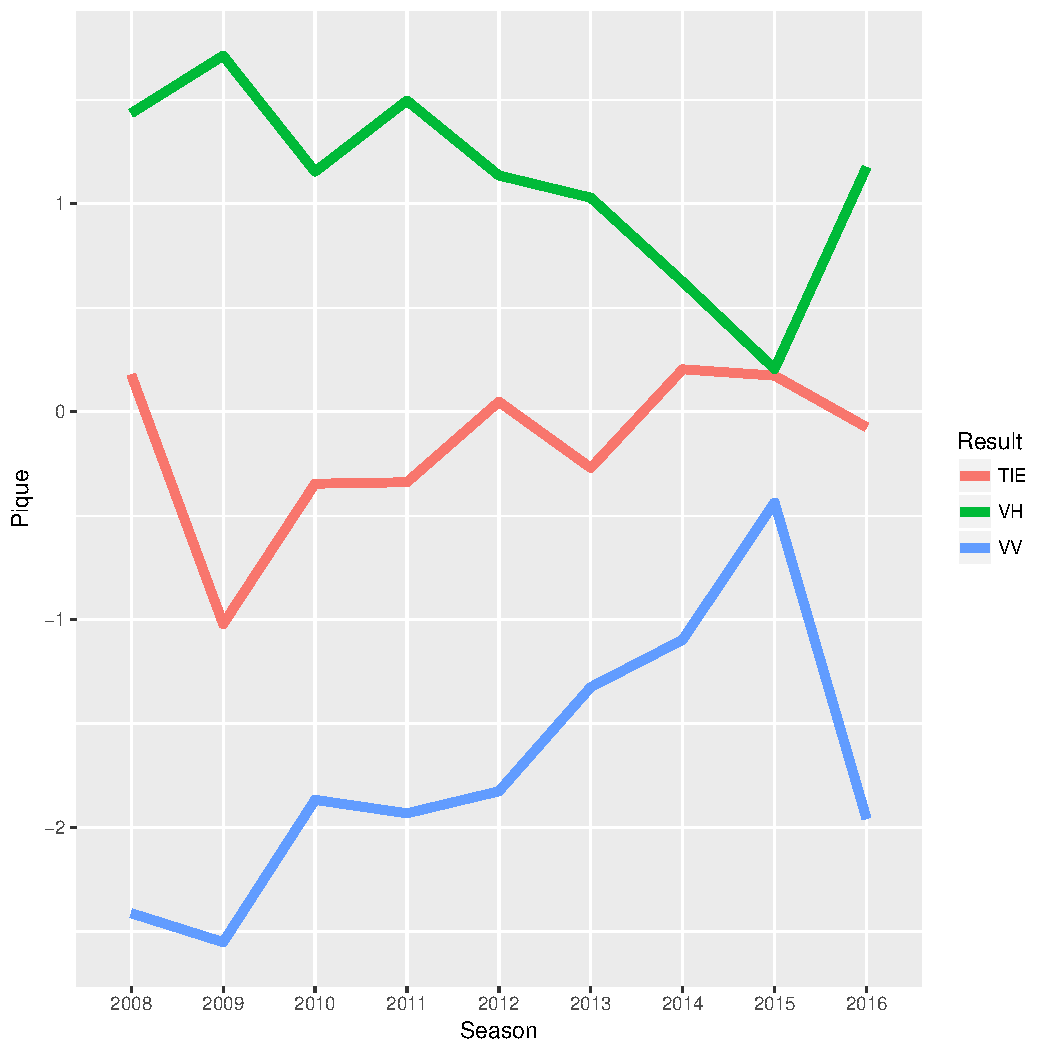
\includegraphics[width=25mm]{pique_result}  & 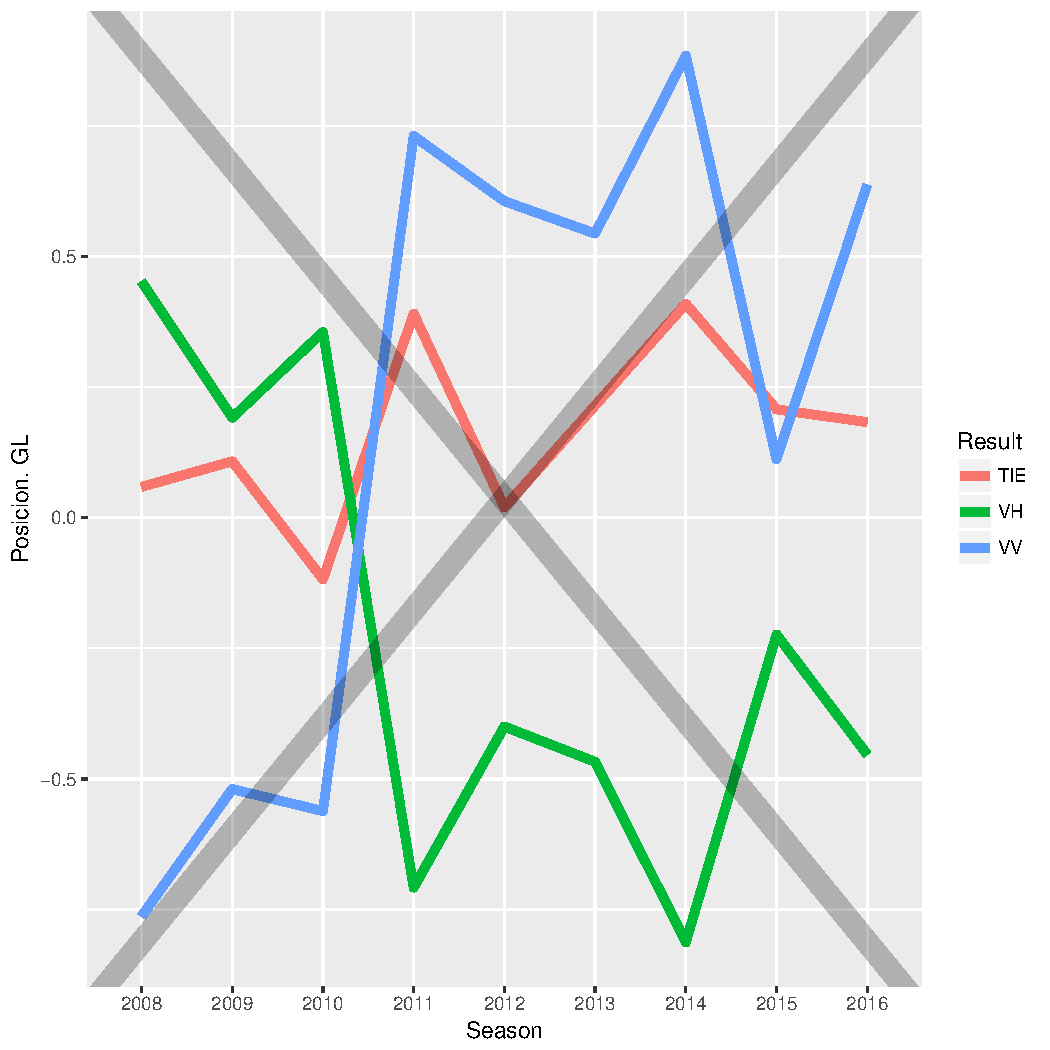
\includegraphics[width=25mm]{posicion_gl_result} &   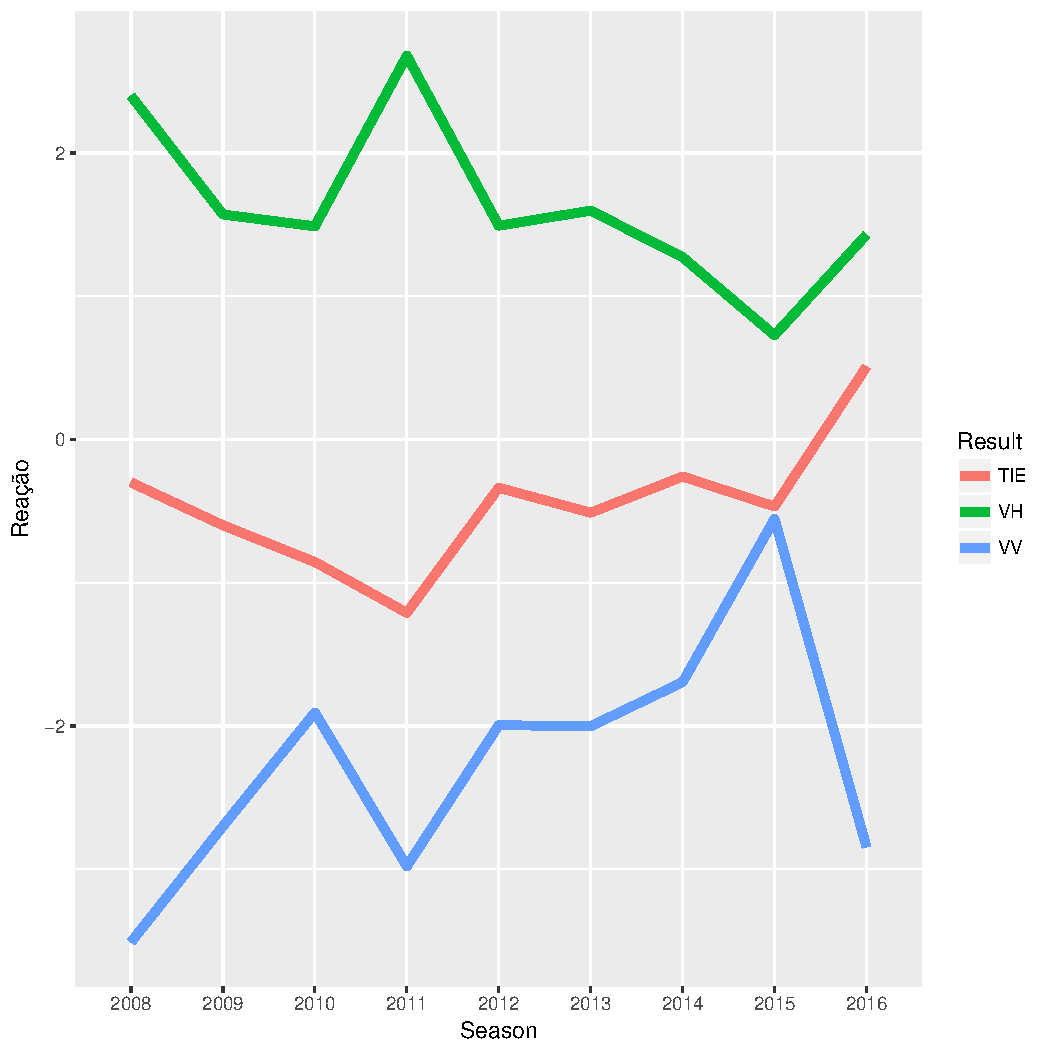
\includegraphics[width=25mm]{reacao_result}&
  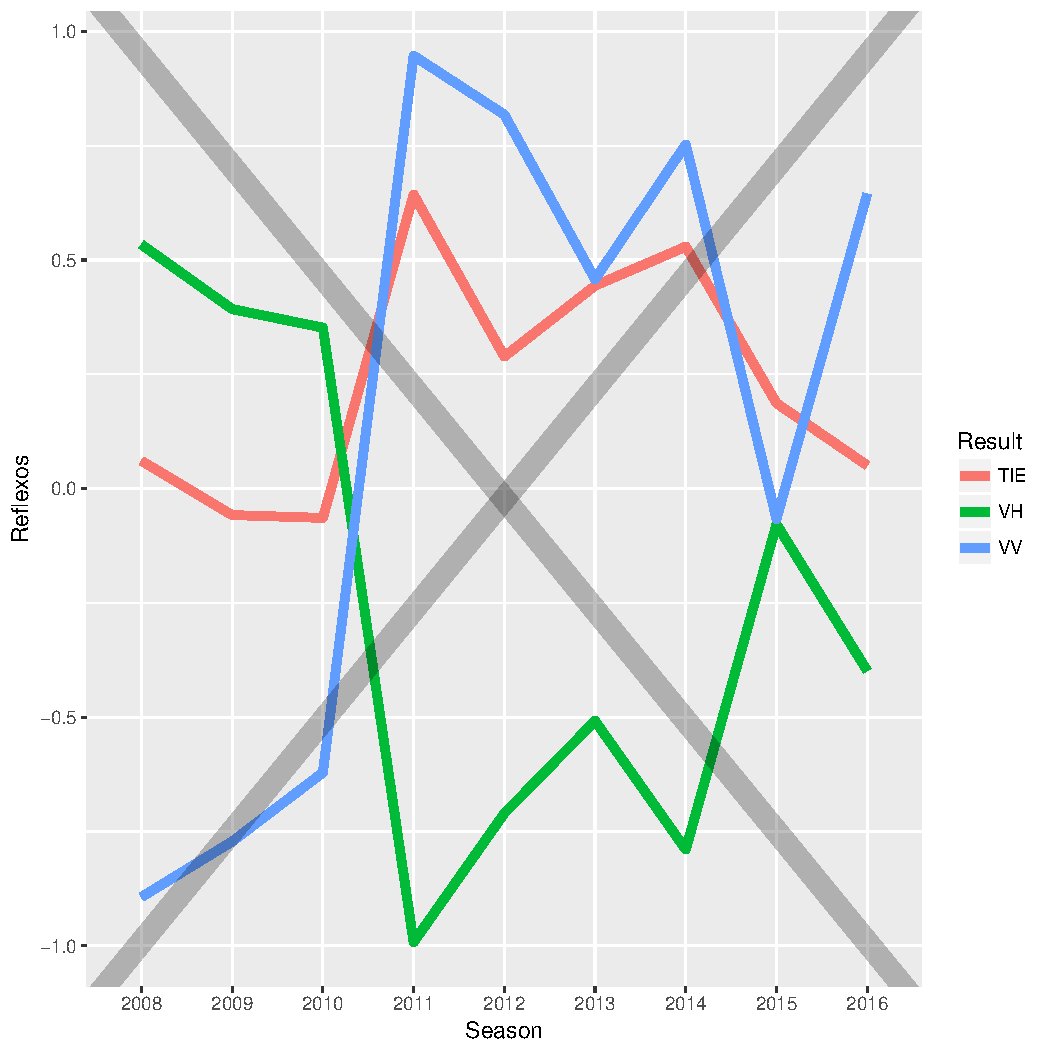
\includegraphics[width=25mm]{reflexos_result}    &    \\
 \scriptsize{(z) pique} & \scriptsize{(aa) posição do goleiro} & \scriptsize{(ab) reação} & \scriptsize{(ac) reflexo} & \\[3pt]

\end{tabular}
    \caption[\scriptsize{Medidas resumo.}]{\scriptsize{Medidas resumo alongo dos anos para cada variável disponível.}}
\end{figure}




 
\section{Considerações finais}
\label{sec:conclu}
\noindent

\bibliographystyle{apacite}
\bibliography{bibli}


\end{document}
